% This file was converted to LaTeX by Writer2LaTeX ver. 1.4
% see http://writer2latex.sourceforge.net for more info
\documentclass[12pt]{article}
\usepackage[utf8]{inputenc}
\usepackage[T1]{fontenc}
\usepackage[english]{babel}
\usepackage{amsmath}
\usepackage{amssymb,amsfonts,textcomp}
\usepackage{array}
\usepackage{supertabular}
\usepackage{hhline}
\usepackage{hyperref}
\hypersetup{colorlinks=true, linkcolor=blue, citecolor=blue, filecolor=blue, urlcolor=blue}
\usepackage{graphicx}
% footnotes configuration
\makeatletter
\renewcommand\thefootnote{\arabic{footnote}}
\makeatother
\newcommand\textsubscript[1]{\ensuremath{{}_{\text{#1}}}}
% Text styles
\newcommand\textstyleListLabeli[1]{\textmd{\textup{#1}}}
\newcommand\textstyleTextonotapieCar[1]{{\fontsize{10pt}{12.0pt}\selectfont \textrm{#1}}}
\newcommand\textstyleFootnoteSymbol[1]{{\fontsize{6.5pt}{7.8pt}\selectfont #1}}
\newcommand\textstyleNone[1]{#1}
\makeatletter
\newcommand\arraybslash{\let\\\@arraycr}
\makeatother
\raggedbottom
% Paragraph styles
\renewcommand\familydefault{\rmdefault}
\newenvironment{styleStandard}{\setlength\leftskip{0cm}\setlength\rightskip{0cm plus 1fil}\setlength\parindent{0cm}\setlength\parfillskip{0pt plus 1fil}\setlength\parskip{0in plus 1pt}\writerlistparindent\writerlistleftskip\leavevmode\normalfont\normalsize\writerlistlabel\ignorespaces}{\unskip\vspace{0.111in plus 0.0111in}\par}
\newenvironment{stylelsAbstract}{\setlength\leftskip{0.5in}\setlength\rightskip{0.5in}\setlength\parindent{0in}\setlength\parfillskip{0pt plus 1fil}\setlength\parskip{0in plus 1pt}\writerlistparindent\writerlistleftskip\leavevmode\normalfont\normalsize\itshape\writerlistlabel\ignorespaces}{\unskip\vspace{0.111in plus 0.0111in}\par}
\newenvironment{stylelsSectioni}{\setlength\leftskip{0.25in}\setlength\rightskip{0in plus 1fil}\setlength\parindent{0in}\setlength\parfillskip{0pt plus 1fil}\setlength\parskip{0.1665in plus 0.016649999in}\writerlistparindent\writerlistleftskip\leavevmode\normalfont\normalsize\fontsize{18pt}{21.6pt}\selectfont\bfseries\writerlistlabel\ignorespaces}{\unskip\vspace{0.0835in plus 0.00835in}\par}
\newenvironment{stylelsSectionii}{\setlength\leftskip{0.25in}\setlength\rightskip{0in plus 1fil}\setlength\parindent{0in}\setlength\parfillskip{0pt plus 1fil}\setlength\parskip{0.222in plus 0.0222in}\writerlistparindent\writerlistleftskip\leavevmode\normalfont\normalsize\fontsize{16pt}{19.2pt}\selectfont\bfseries\writerlistlabel\ignorespaces}{\unskip\vspace{0.0835in plus 0.00835in}\par}
\newenvironment{stylelsLanginfo}{\renewcommand\baselinestretch{1.0}\setlength\leftskip{0.0783in}\setlength\rightskip{0in plus 1fil}\setlength\parindent{0in}\setlength\parfillskip{0pt plus 1fil}\setlength\parskip{0in plus 1pt}\writerlistparindent\writerlistleftskip\leavevmode\normalfont\normalsize\writerlistlabel\ignorespaces}{\unskip\vspace{0in plus 1pt}\par}
\newenvironment{styleDefault}{\renewcommand\baselinestretch{1.0}\setlength\leftskip{0cm}\setlength\rightskip{0cm plus 1fil}\setlength\parindent{0cm}\setlength\parfillskip{0pt plus 1fil}\setlength\parskip{0in plus 1pt}\writerlistparindent\writerlistleftskip\leavevmode\normalfont\normalsize\writerlistlabel\ignorespaces}{\unskip\vspace{0in plus 1pt}\par}
\newenvironment{styleBody}{\renewcommand\baselinestretch{1.0}\setlength\leftskip{0cm}\setlength\rightskip{0cm plus 1fil}\setlength\parindent{0cm}\setlength\parfillskip{0pt plus 1fil}\setlength\parskip{0in plus 1pt}\writerlistparindent\writerlistleftskip\leavevmode\normalfont\normalsize\writerlistlabel\ignorespaces}{\unskip\vspace{0in plus 1pt}\par}
\newenvironment{styleBibliography}{\setlength\leftskip{0.5in}\setlength\rightskip{0in plus 1fil}\setlength\parindent{-0.5in}\setlength\parfillskip{0pt plus 1fil}\setlength\parskip{0in plus 1pt}\writerlistparindent\writerlistleftskip\leavevmode\normalfont\normalsize\writerlistlabel\ignorespaces}{\unskip\vspace{0in plus 1pt}\par}
% List styles
\newcommand\writerlistleftskip{}
\newcommand\writerlistparindent{}
\newcommand\writerlistlabel{}
\newcommand\writerlistremovelabel{\aftergroup\let\aftergroup\writerlistparindent\aftergroup\relax\aftergroup\let\aftergroup\writerlistlabel\aftergroup\relax}
\newcounter{listWWNumxxiileveli}
\newcounter{listWWNumxxiilevelii}[listWWNumxxiileveli]
\newcounter{listWWNumxxiileveliii}[listWWNumxxiilevelii]
\newcounter{listWWNumxxiileveliv}[listWWNumxxiileveliii]
\renewcommand\thelistWWNumxxiileveli{\arabic{listWWNumxxiileveli}}
\renewcommand\thelistWWNumxxiilevelii{\arabic{listWWNumxxiileveli}.\arabic{listWWNumxxiilevelii}}
\renewcommand\thelistWWNumxxiileveliii{\arabic{listWWNumxxiileveli}.\arabic{listWWNumxxiilevelii}.\arabic{listWWNumxxiileveliii}}
\renewcommand\thelistWWNumxxiileveliv{\arabic{listWWNumxxiileveli}.\arabic{listWWNumxxiilevelii}.\arabic{listWWNumxxiileveliii}.\arabic{listWWNumxxiileveliv}}
\newcommand\labellistWWNumxxiileveli{\thelistWWNumxxiileveli.}
\newcommand\labellistWWNumxxiilevelii{\thelistWWNumxxiilevelii.}
\newcommand\labellistWWNumxxiileveliii{\thelistWWNumxxiileveliii.}
\newcommand\labellistWWNumxxiileveliv{\thelistWWNumxxiileveliv.}
\newenvironment{listWWNumxxiileveli}{\def\writerlistleftskip{\setlength\leftskip{2.75in}}\def\writerlistparindent{}\def\writerlistlabel{}\def\item{\def\writerlistparindent{\setlength\parindent{-0.25in}}\def\writerlistlabel{\stepcounter{listWWNumxxiileveli}\makebox[0cm][l]{\labellistWWNumxxiileveli}\hspace{-6.35cm}\writerlistremovelabel}}}{}
\newenvironment{listWWNumxxiilevelii}{\def\writerlistleftskip{\setlength\leftskip{1in}}\def\writerlistparindent{}\def\writerlistlabel{}\def\item{\def\writerlistparindent{\setlength\parindent{-0.25in}}\def\writerlistlabel{\stepcounter{listWWNumxxiilevelii}\makebox[0cm][l]{\labellistWWNumxxiilevelii}\hspace{-1.905cm}\writerlistremovelabel}}}{}
\newenvironment{listWWNumxxiileveliii}{\def\writerlistleftskip{\setlength\leftskip{1.5in}}\def\writerlistparindent{}\def\writerlistlabel{}\def\item{\def\writerlistparindent{\setlength\parindent{-0.1252in}}\def\writerlistlabel{\stepcounter{listWWNumxxiileveliii}\makebox[0cm][r]{\labellistWWNumxxiileveliii}\hspace{-3.4919918cm}\writerlistremovelabel}}}{}
\newenvironment{listWWNumxxiileveliv}{\def\writerlistleftskip{\setlength\leftskip{2in}}\def\writerlistparindent{}\def\writerlistlabel{}\def\item{\def\writerlistparindent{\setlength\parindent{-0.25in}}\def\writerlistlabel{\stepcounter{listWWNumxxiileveliv}\makebox[0cm][l]{\labellistWWNumxxiileveliv}\hspace{-4.4449997cm}\writerlistremovelabel}}}{}
\newcounter{listWWNumiileveli}
\newcounter{listWWNumiilevelii}[listWWNumiileveli]
\newcounter{listWWNumiileveliii}[listWWNumiilevelii]
\newcounter{listWWNumiileveliv}[listWWNumiileveliii]
\renewcommand\thelistWWNumiileveli{\arabic{listWWNumiileveli}}
\renewcommand\thelistWWNumiilevelii{\alph{listWWNumiilevelii}}
\renewcommand\thelistWWNumiileveliii{}
\renewcommand\thelistWWNumiileveliv{}
\newcommand\labellistWWNumiileveli{\textstyleListLabeli{(\thelistWWNumiileveli)}}
\newcommand\labellistWWNumiilevelii{\thelistWWNumiilevelii.}
\newcommand\labellistWWNumiileveliii{\thelistWWNumiileveliii}
\newcommand\labellistWWNumiileveliv{\thelistWWNumiileveliv}
\newenvironment{listWWNumiileveli}{\def\writerlistleftskip{\setlength\leftskip{0.3217in}}\def\writerlistparindent{}\def\writerlistlabel{}\def\item{\def\writerlistparindent{\setlength\parindent{-0.1965in}}\def\writerlistlabel{\stepcounter{listWWNumiileveli}\makebox[0cm][l]{\labellistWWNumiileveli}\hspace{0.0783in}\writerlistremovelabel}}}{}
\newenvironment{listWWNumiilevelii}{\def\writerlistleftskip{\setlength\leftskip{2.1339in}}\def\writerlistparindent{}\def\writerlistlabel{}\def\item{\def\writerlistparindent{\setlength\parindent{0.5516in}}\def\writerlistlabel{\stepcounter{listWWNumiilevelii}\makebox[0cm][l]{\labellistWWNumiilevelii}\hspace{-0.6694in}\writerlistremovelabel}}}{}
\newenvironment{listWWNumiileveliii}{\def\writerlistleftskip{\setlength\leftskip{2.1339in}}\def\writerlistparindent{}\def\writerlistlabel{}\def\item{\def\writerlistparindent{\setlength\parindent{-0.1965in}}\def\writerlistlabel{\stepcounter{listWWNumiileveliii}\labellistWWNumiileveliii\writerlistremovelabel}}}{}
\newenvironment{listWWNumiileveliv}{\def\writerlistleftskip{\setlength\leftskip{2.1339in}}\def\writerlistparindent{}\def\writerlistlabel{}\def\item{\def\writerlistparindent{\setlength\parindent{-0.1965in}}\def\writerlistlabel{\stepcounter{listWWNumiileveliv}\labellistWWNumiileveliv\writerlistremovelabel}}}{}
\setlength\tabcolsep{1mm}
\renewcommand\arraystretch{1.3}
\title{}
\author{Anna}
\date{2019-07-23}
\begin{document}
\title{\textsuperscript{The lexical underspecification of Bantu causatives and applicatives}}
\maketitle

\begin{styleStandard}
\textbf{Mattie Wechsler}
\end{styleStandard}

\begin{styleStandard}
\textbf{(Independent researcher)}
\end{styleStandard}

\begin{stylelsAbstract}
Abstract. This paper presents original evidence for an additional merge location and semantic interpretation of Bantu applicatives, drawing on complex multiply applicativized and causativized constructions for empirical support. The paper also identifies and discusses challenging data from Bantu causatives. Previous analyses of causative and applicative constructions in the world’s languages have enumerated different kinds of causative and applicative heads, stored separately in the lexicon, each with their own particular selectional requirements. 
\end{stylelsAbstract}

\begin{stylelsAbstract}
As the number of attested structural positions, potential compliments, and semantic interpretations for these heads grow in the literature, however, the model bloats and becomes less compelling. I ultimately adopt recent analysis from Wood \& Marantz (2017) and assert that a single underspecified argument introducer is sufficient to account for the Bantu data I present. \ In order to accommodate the new theory of argument introduction, I also propose a new, more semantically-oriented, model of causative compliment selection. 
\end{stylelsAbstract}


\setcounter{listWWNumxxiileveli}{0}
\begin{listWWNumxxiileveli}
\item 
\begin{stylelsSectioni}
Introduction
\end{stylelsSectioni}
\end{listWWNumxxiileveli}
\begin{styleStandard}
For my analysis, I assume that even in languages without explicit applicative morphology, applicative argument-introducing heads are responsible for the additional arguments in dative/ditransitive/double-object constructions.\textsc{ }Therefore, while this paper occurs in the applicative section of a volume on dative structures, my analysis will not make use of, or rely on, this distinction. 
\end{styleStandard}

\begin{styleStandard}
In this paper I argue that evidence from Bantu supports a model with fewer argument introducers available in the lexicon than previous accounts (most prominently, Pylkkänen 2008) have suggested. My analysis makes heavy use of Wood \& Marantz's (2017) work, which argues similarly for a radically reduced inventory of argument-introducing heads. 
\end{styleStandard}

\begin{styleStandard}
In §2, I present challenging data from Bantu causatives. Ultimately, I argue that causatives are underspecified for categorial compliment selection, and I propose an original treatment of cross-linguistic variation in causative constructions.
\end{styleStandard}

\begin{styleStandard}
In §3, I structure my analysis around the assumption that all applicatives are underlyingly the same as one another, as well as all other non-core\textsc{ }argument\textsc{ }introducers. I demonstrate that the same applicative surface structure often corresponds to multiple underlying structures, and I also present original evidence for an additional applicative merge-location in Shona. 
\end{styleStandard}

\begin{styleStandard}
In §4, I acknowledge a few sticking points in the analysis, speculate about some unanswered questions, and identify fruitful areas for further research on the topics and issues plumbed in this paper. 
\end{styleStandard}

\begin{listWWNumxxiileveli}
\item 
\begin{stylelsSectioni}
Causatives
\end{stylelsSectioni}

\begin{listWWNumxxiilevelii}
\item 
\begin{stylelsSectionii}
Data from Bantu 
\end{stylelsSectionii}
\end{listWWNumxxiilevelii}
\end{listWWNumxxiileveli}
\begin{styleStandard}
Consider the following:
\end{styleStandard}


\setcounter{listWWNumiileveli}{0}
\begin{listWWNumiileveli}
\item 
\begin{stylelsLanginfo}
\label{bkm:Ref515937112}Shona
\end{stylelsLanginfo}
\end{listWWNumiileveli}
\begin{flushleft}
\tablefirsthead{}
\tablehead{}
\tabletail{}
\tablelasttail{}
\begin{supertabular}{m{0.22885984in}m{0.9205598in}m{1.1087599in}m{0.29625985in}m{0.026159845in}m{0.6913598in}m{-0.01554016in}m{0.6712598in}}
a. &
\textit{Tinotenda} &
\multicolumn{6}{m{3.1719599in}}{\textit{a-nyur-a}}\\
 &
1.Tinotenda \  &
\multicolumn{6}{m{3.1719599in}}{\textsc{sm1-}drown\textsc{{}-fv}}\\
 &
\multicolumn{4}{m{2.5879598in}}{‘Tinotenda drowned.’} &
\multicolumn{2}{m{0.7545598in}}{} &
\\
b. &
*\textit{Tinotenda} &
\textit{a-nyur-a} &
\multicolumn{4}{m{1.2344599in}}{\textit{ne-kuda}} &
\\
 &
1.Tinotenda \  &
\textsc{sm1-}drown\textsc{{}-fv} &
\multicolumn{4}{m{1.2344599in}}{with-love} &
\\
 &
\multicolumn{4}{m{2.5879598in}}{‘Tinotenda drowned intentionally.’ } &
\multicolumn{2}{m{0.7545598in}}{} &
\\
c. &
\textit{Tinotenda} &
\multicolumn{2}{m{1.4837599in}}{\textit{a-nyur-is-a}} &
\multicolumn{2}{m{0.7962598in}}{\textit{Tatenda}} &
\multicolumn{2}{m{0.7344598in}}{\textit{ne-kuda}}\\
 &
1.Tinotenda \  &
\multicolumn{2}{m{1.4837599in}}{\textsc{sm1-}drown\textsc{{}-caus-fv}} &
\multicolumn{2}{m{0.7962598in}}{1.Tatenda} &
\multicolumn{2}{m{0.7344598in}}{with-love}\\
 &
\multicolumn{6}{m{3.4212599in}}{‘Tinotenda drowned Tatenda intentionally.’} &
\\
\end{supertabular}
\end{flushleft}
\begin{listWWNumiileveli}
\item 
\begin{stylelsLanginfo}
\label{bkm:Ref516385492}Shona
\end{stylelsLanginfo}
\end{listWWNumiileveli}
\begin{flushleft}
\tablefirsthead{}
\tablehead{}
\tabletail{}
\tablelasttail{}
\begin{supertabular}{m{0.21365985in}m{0.9205598in}m{1.2337599in}m{0.29625985in}m{0.7337598in}m{0.7344598in}}
a. &
\textit{Tinotenda} &
\textit{a-ka-yimb-a \ \ \ \ \ \ \ \ \ \ \ \ \ \ } &
\multicolumn{3}{m{1.9219599in}}{\textit{ne-kuda}}\\
 &
1.Tinotenda &
\textsc{sm1-pst-}sing\textsc{{}-fv} &
\multicolumn{3}{m{1.9219599in}}{with-love}\\
 &
\multicolumn{3}{m{2.60806in}}{‘Tinotenda sang intentionally.’} &
\multicolumn{2}{m{1.5469599in}}{}\\
b. &
\textit{Tinotenda} &
\multicolumn{2}{m{1.6087599in}}{\textit{a-ka-yimb-is-a}} &
\textit{Tatenda} &
\textit{ne-kuda}\\
 &
1.Tinotenda \  &
\multicolumn{2}{m{1.6087599in}}{\textsc{sm1-pst-}sing\textsc{{}-caus-fv}} &
1.Tatenda &
with-love\\
 &
\multicolumn{5}{m{4.23376in}}{i.‘Tinotenda intentionally made Tatenda sing.’ 

ii. *‘Tinotenda made Tatenda intentionally sing.’}\\
\end{supertabular}
\end{flushleft}
\begin{styleDefault}
In \ causativization appears to “add” an Agent to a structure without one.\footnote{ In describing causative alternations, it is easy to lean on metaphor that conflates theory. Within the theoretical framework of this paper, it is not considered to be the case that causative constructions are formed by applying a transformational causative process to an already generated non-causative sentence. When I discuss what a causative head “adds to” or “subtracts from” a structure, I’m not referring to the cognitive process of causativization as it occurs in a speaker’s mind when their native grammar generates a causative construction, but to the comparison of two already generated sentences in an alternation. For literal descriptions of grammatical processes, I use words like “introduce” or “merge”.} Superficially,(\ref{bkm:Ref516385492}) looks the same. In (\ref{bkm:Ref516385492}), however, only the Causer is an Agent, which would imply that causativization in one case entails the “addition” of an Agent and in another, both the “addition” and “subtraction” of an Agent.
\end{styleDefault}

\begin{styleDefault}
It is difficult to ascribe a single syntactic function to Shona causatives, because the differences exhibited between causative constructions and their non-causative counterparts are not consistent. \ Pylkkänen (2008) grapples with the same conundrum, but cross-linguistically. Her typological proposal distinguishes based on two variables, merge height and a property she calls \textsc{voice-bundling. }Causatives either select as their complement VoiceP \ (\textsc{phase-selecting)}, vP \textsc{(verb-selecting)}, or the verb root ${\surd}$ (\textsc{root-selecting)}. Additionally, causatives are either of the Voice-bundling type, meaning that they merge with Voice to create a single Agent-introducing head, or they are of the Non-Voice-bundling type, meaning that they merge as a free head in the structure and are not syntactically bound to Voice. 
\end{styleDefault}

\begin{styleDefault}
For Pylkkänen (and for my analysis), causatives are not argument introducers. They introduce a causative meaning and a syntactic relationship between an Agent (introduced by Voice) and the event conveyed by the verb phrase. Pylkkänen makes this distinction because some languages allow causative constructions without an overt Causer role. In languages with the Voice-bundling type of causative, however, this split is all but irrelevant because Voice-bundled causatives constitute a single Causer-introducing head. 
\end{styleDefault}

\begin{styleDefault}
Because verb-selecting causatives merge below Voice, and Voice is the only head that introduces Agents, the subject is the only agentive argument. Phase-selecting causatives are merged above Voice and allow for two agentive arguments. Agent-oriented modification of the Causee diagnoses the merge location of the causative. The possible interpretations in (\ref{bkm:Ref516385492})\ show that Shona causative constructions have only one agentive argument and therefore do not merge above Voice. In this respect, Shona is unlike Venda, which according to Pylkkänen has phase-selecting causatives:
\end{styleDefault}

\begin{listWWNumiileveli}
\item 
\begin{stylelsLanginfo}
\label{bkm:Ref516386347}Venda (Pylkkänen 2008:83)
\end{stylelsLanginfo}
\end{listWWNumiileveli}
\begin{flushleft}
\tablefirsthead{}
\tablehead{}
\tabletail{}
\tablelasttail{}
\begin{supertabular}{m{1.0254599in}m{1.3170599in}m{0.7754598in}m{0.6087598in}m{0.42125985in}m{1.0462599in}}
{\itshape Muuhambadz} &
\textit{o-reng-is-a \ \ \ \ \ \ \ \ \ \ \ \ \ \ \ \ } &
{\itshape Katonga} &
{\itshape modoro} &
{\itshape nga} &
{\itshape dzangalelo}\\
1.salesman \ \ \ \textsc{\ } &
\textsc{sm1}{}-buy-\textsc{caus}{}-\textsc{fv }\ \  &
1.Katonga &
9.car &
with &
10.enthusiasm\\
\multicolumn{5}{m{4.46296in}}{i. ‘The salesman eagerly made Katonga buy the car.’

ii. ‘The salesman made Katonga eagerly buy the car.’} &
\\
\end{supertabular}
\end{flushleft}
\begin{styleDefault}
In (\ref{bkm:Ref516386347})\ ‘eagerly’ can modify either ‘the salesman’ or ‘Katonga’, therefore indicating that in Venda causatives merge above Voice. \ 
\end{styleDefault}

\begin{styleDefault}
Pylkkänen’s typology offers an explanation for the difference between (\ref{bkm:Ref516385492})\ and (\ref{bkm:Ref516386347}), but it leaves an important question unanswered: what head introduces the non-agentive Causee when Voice introduces Agents exclusively? Causative constructions with non-agentive Causees are cross-linguistically common (Kulikov 2001; Kittilä 2013), so this gap in the theory is not insignificant. Pylkkänen acknowledges this shortfall but does not seek to address it in her anlaysis (2008:107). I do seek to address it, and I propose a solution in §2.2. \ 
\end{styleDefault}

\begin{styleDefault}
While this structural puzzle does not apply to languages with phase-selecting causatives, like Venda, such languages do pose a related problem:
\end{styleDefault}

\begin{listWWNumiileveli}
\item 
\begin{stylelsLanginfo}
\label{bkm:Ref516386444}Venda Pylkkänen (2008: 2)
\end{stylelsLanginfo}
\end{listWWNumiileveli}
\begin{flushleft}
\tablefirsthead{}
\tablehead{}
\tabletail{}
\tablelasttail{}
\begin{supertabular}{m{0.22335985in}m{0.6712598in}m{-0.01554016in}m{0.8580598in}m{0.42125985in}m{0.6087598in}}
a. &
{\itshape Mahada} &
\multicolumn{2}{m{0.9212598in}}{\textit{o-nok-a}} &
\multicolumn{2}{m{1.1087599in}}{}\\
 &
6. snow \  &
\multicolumn{2}{m{0.9212598in}}{\textsc{sm1}{}-melt-\textsc{fv }} &
\multicolumn{2}{m{1.1087599in}}{}\\
 &
\multicolumn{3}{m{1.6712599in}}{‘The snow melted.’} &
\multicolumn{2}{m{1.1087599in}}{}\\
b. &
\multicolumn{2}{m{0.7344598in}}{{\itshape Mukasa}} &
\multicolumn{2}{m{1.3580599in}}{{\itshape o-nok-is-a \ \ \ \ \ \ \ \ \ \ \ \ \ \ \ \ \ \ \ }} &
{\itshape mahada}\\
 &
\multicolumn{2}{m{0.7344598in}}{1.Mukasa \ } &
\multicolumn{2}{m{1.3580599in}}{\textsc{sm1}{}-melt-\textsc{caus}{}-\textsc{fv }} &
6.snow\\
 &
\multicolumn{5}{m{2.8587599in}}{‘Mukasa melted the snow.’}\\
\end{supertabular}
\end{flushleft}
\begin{styleDefault}
Venda’s phase-selecting causative supposedly needs to merge with Voice, but Voice is not present in the Agent-lacking unaccusative construction in (\ref{bkm:Ref516386444}). \ 
\end{styleDefault}

\begin{styleDefault}
The data in (\ref{bkm:Ref516386347}){}-(\ref{bkm:Ref516386444}) shows that in both Venda and Shona causatives merge with more than one kind of compliment. Furthermore, flexible selectional requirements do not appear to be atypical of Bantu causatives: 
\end{styleDefault}

\begin{listWWNumiileveli}
\item 
\begin{stylelsLanginfo}
Bemba (Givón 1976, 329: 18 via Pylkkänen 2008: 115)
\end{stylelsLanginfo}
\end{listWWNumiileveli}
\begin{flushleft}
\tablefirsthead{}
\tablehead{}
\tabletail{}
\tablelasttail{}
\begin{supertabular}{m{2.0983598in}m{0.8587598in}m{0.7337598in}m{0.8587598in}}
{\itshape Naa-mu-fu-und-ishya} &
\textit{uku-laanda} &
{\itshape iciBemba} &
{\itshape ku-mufulo}\\
\textsc{sm}1\textsc{{}-pst-om1}{}-learn-\textsc{caus-fv} &
\textsc{inf-}speak &
4.Bemba &
on-purpose\\
\multicolumn{3}{m{3.8483598in}}{i. ‘I, on purpose, made him learn to speak Bemba.’

ii. *‘I made him on purpose learn to speak Bemba.’} &
\\
\end{supertabular}
\end{flushleft}
\begin{listWWNumiileveli}
\item 
\begin{stylelsLanginfo}
\label{bkm:Ref516386265}Bemba (Givón 1969: 155)
\end{stylelsLanginfo}
\end{listWWNumiileveli}
\begin{flushleft}
\tablefirsthead{}
\tablehead{}
\tabletail{}
\tablelasttail{}
\begin{supertabular}{m{0.37615985in}m{0.52335984in}m{0.35875985in}m{1.4837599in}m{0.046259843in}m{0.7962598in}}
a. &
\multicolumn{2}{m{0.96085984in}}{{\itshape Aba-Bemba}} &
\multicolumn{2}{m{1.6087599in}}{\textit{ba-ali-ful-a}} &
\\
 &
\multicolumn{2}{m{0.96085984in}}{all-2.Bemba \ } &
\multicolumn{2}{m{1.6087599in}}{\textsc{sm2}{}-\textsc{prog}{}-multiply-\textsc{fv}} &
\\
 &
\multicolumn{4}{m{2.6483598in}}{‘The Bemba people multiplied.’} &
\\
b. &
{\itshape Leesa} &
\multicolumn{2}{m{1.9212599in}}{{\itshape a-a-fu-shy-a }} &
\multicolumn{2}{m{0.9212598in}}{{\itshape aba-Bemba}}\\
 &
1.God  &
\multicolumn{2}{m{1.9212599in}}{\textsc{sm1-pst}{}-multiply-\textsc{caus}{}-\textsc{fv}} &
\multicolumn{2}{m{0.9212598in}}{all-2.Bemba}\\
 &
\multicolumn{5}{m{3.5233598in}}{‘God multiplied the Bemba people.’}\\
\end{supertabular}
\end{flushleft}
\begin{styleDefault}
Bemba demonstrates the same variation in causative complement selection as Shona, embedding unaccusative structures, as well as non-agentive external arguments in unergative and transitive verb phrases. 
\end{styleDefault}

\begin{styleStandard}
Kim (2011) argues that in causativized transitive and unergative structures, non-agentive Causees are introduced by unpronounced high applicative\textsc{ }heads (see §3 for a detailed explanation of low and high \textsc{appl).} This proposal is economical in that high applicative heads are available in the lexicon of Bantu languages (and Korean, from which Kim draws her evidence for the solution), they merge in between Voice and the verb, and they are associated with non-agentive arguments. Furthermore, though it is irrelevant to the Bantu data, Korean Causees are dative arguments, that is, they pattern with the distribution and morphological marking of applied/indirect objects, such as Benefactives and Recipients (Kim 2011).\footnote{\textstyleTextonotapieCar{ Although Bantu does not have any morphological case marking, I want to take this opportunity to clarify this paper's stance on abstract Case in Bantu. I do not adopt recent analysis from }\textstyleTextonotapieCar{Diercks (2012), who argues that Bantu languages parametrically opt out of abstract Case-licensing en masse. I assume that the arguments in my Bantu data require abstract Case-licensing (see }\textstyleTextonotapieCar{van der Wal 2015, }\textstyleTextonotapieCar{Sheehan \& van der Wal 2016, }\textstyleTextonotapieCar{Halpert 2012, and }\textstyleTextonotapieCar{Wechsler 2014, 2016 for}\textrm{ }\textstyleTextonotapieCar{evidence of Case features in Bantu). I am unable to devote the analysis in this paper towards identifying a licensing head for each argument, but I consider further research into \textit{i}*’s role in Case-licensing to be an important next step in assessing the utility and feasibility of this analysis.}\textrm{ }\par } 
\end{styleStandard}

\begin{styleDefault}
In Pylkkänen’s model of argument introduction, however, these various causative heads are all separate lexical items, specified each for a particular selectional requirement, and acquired by any given language from a universal inventory. Kim’s proposal adds another head (two, if it also comes in Voice-bundling and Non-Voice-bundling varieties), an applicative-selecting causative, to both Pylkkänen’s universal inventory, and to any given language with causative diversity similar to that of Shona and Bemba. The resulting system is congested, and I assert that the causative data in (\ref{bkm:Ref515937112}){}-(\ref{bkm:Ref516386265}) provide an opportunity to simplify both the lexicons of the individual languages as well as the universal inventory. \newline
\newline
Rather than an inventory of 6-8 distinct causative heads, from which many languages would have to select multiple items to account for their range of causative diversity, I argue that causative heads specified for a maximum compliment size offer a better solution. This proposal captures the fact that causativized unnaccusative structures occur both in languages with Voice-selecting and verb/applicative-selecting causatives, despite unaccusatives apparently contradicting selectional requirements for larger compliments. The notion that causatives have an upper-limit, rather than one categorial mandate is intuitive, and my analysis is reminiscent of a similar proposal, made by Haspelmath (2016) involving his concept of the “spontaneity scale”. \newline

\end{styleDefault}

\begin{styleStandard}
§2.2 focuses on clarifying this paper’s treatment of argument introducers, drawing heavily on Wood \& Marantz (2017). Their proposal has serious implications for the mechanics involved in causative compliment selection, but by building on the notion of “compliment size” and formulating a more specific definition of that concept, I am able to better accommodate both the new theory and the data. I also use Wood \& Marantz’s analysis to make a proposal about the identity of the head responsible for introducing non-agentive Causees in constructions like those in (\ref{bkm:Ref516385492})\ and (\ref{bkm:Ref516386265}).
\end{styleStandard}


\setcounter{listWWNumxxiileveli}{0}
\begin{listWWNumxxiileveli}
\item 

\setcounter{listWWNumxxiilevelii}{0}
\begin{listWWNumxxiilevelii}
\item 
\begin{stylelsSectionii}
Wood \& Marantz’s \textit{i}*
\end{stylelsSectionii}
\end{listWWNumxxiilevelii}
\end{listWWNumxxiileveli}
\begin{styleDefault}
Wood and Marantz (2017) assert that all non-core\textsc{ }arguments in any language are introduced by the same underspecified head, “\textit{i}*”. They provide a distinct syntactic structure for Voice, low and high applicative heads, and prepositional heads, little p and big P, arguing that if syntax can account for the difference between these semantically varying instances of argument introduction, then it is redundant to have the lexicon store categorially separate heads. 
\end{styleDefault}

\begin{styleDefault}
Voice is simply the product of \textit{i}* merging with the verbalizing head little v and allowing for the introduction of an external agentive argument. Figure 1, adapted from their work (2017: 261), demonstrates this structure.
\end{styleDefault}

\begin{styleDefault}
\ \   [Warning: Image ignored] % Unhandled or unsupported graphics:
%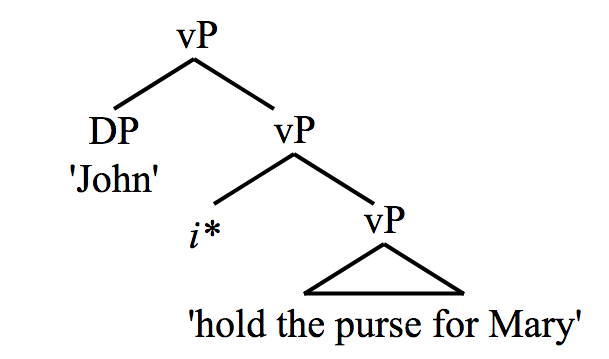
\includegraphics[width=3.0272in,height=1.7827in,width=\textwidth]{wechsler-img001.png}
 
\end{styleDefault}

\begin{styleDefault}
Figure 1: \textit{Wood \& Marantz’s i* introducing an Agent} 
\end{styleDefault}

\begin{styleDefault}
While \textit{i}* \textbf{can} introduce an Agent following its merge with little v, it can also have an expletive interpretation and introduce non-agentive external arguments. The meaning of \textit{i}* can be computed in one of two ways at the syntax-semantics interface. Either \textit{i}* can imbue a relation implied by the semantics of its compliment between the argument it introduces and that compliment (non-expletive), or alternatively it can provide only a means for structural insertion, contributing no semantic “glue” to assist in integrating the argument it introduces (expletive). 
\end{styleDefault}

\begin{styleDefault}
The expletive interpretation is only available when an alternative strategy of semantic integration exists. The Japanese adversity causative, reproduced from Wood \& Marantz in (\ref{bkm:Ref516386625}), demonstrates this point. 
\end{styleDefault}


\setcounter{listWWNumiileveli}{0}
\begin{listWWNumiileveli}
\item 
\begin{stylelsLanginfo}
\label{bkm:Ref516386625}Japanese (Wood \& Marantz 2017: 274)
\end{stylelsLanginfo}
\end{listWWNumiileveli}
\begin{flushleft}
\tablefirsthead{}
\tablehead{}
\tabletail{}
\tablelasttail{}
\begin{supertabular}{m{0.7955598in}m{0.7962598in}m{0.9844598in}}
\textit{Taroo-ga} &
\textit{Musuko-o} &
\textit{si-ase-ta}\\
Taro-\textsc{nom} &
Son-\textsc{acc} &
die-\textsc{caus-pst}\\
\multicolumn{3}{m{2.7337599in}}{i. ‘Taro caused his son to die.’

ii. ‘Taro’s son died on him.’}\\
\end{supertabular}
\end{flushleft}
\begin{styleDefault}
The second possible meaning in (\ref{bkm:Ref516386625}), where \textit{Taro} is negatively affected by his son’s death (but crucially does not play any role in bringing it about), is the adversity causative interpretation. The event of Taro’s son’s death does not necessitate an agentive participant, so \textit{i}* need not necessarily (though it may, as in the first interpretation of (\ref{bkm:Ref516386625})) relate an Agent to that event. As a non-agentive affectee, the \textsc{dp} \textit{Taroo-ga }must be semantically integrated into the structure by some mechanism. Wood \& Marantz argue that, in a structure similar to possessor-raising, \textit{Taroo} is introduced by expletive \textit{i}*, but integrated by saturating a possessor role generated lower down in the \textsc{dp} \textit{musuko-o}. This structure, adapted from a similar rendering in Wood \& Marantz (2017: 274), is approximated in (\ref{bkm:Ref515943970}).
\end{styleDefault}

\begin{listWWNumiileveli}
\item 
\begin{stylelsLanginfo}
\label{bkm:Ref515943970}[Taroo [\textit{i}* [\textsc{vP} die-\textsc{caus} [\textsc{dp} \textsc{possessor} son]]]] 
\end{stylelsLanginfo}
\end{listWWNumiileveli}
\begin{styleDefault}
\ \ \ \ \ \ \ \ \ \ \ \ \ \ \ \   [Warning: Image ignored] % Unhandled or unsupported graphics:
%
\includegraphics[width=2.0634in,height=0.2646in,width=\textwidth]{wechsler-img002.png}
 \ \ \ \ \ \ \ \ \ \ \ \ \ \ \ \ \ 
\end{styleDefault}

\begin{styleDefault}
The arrow in (\ref{bkm:Ref515943970})\ represents the relationship between the possessor role and the argument \textit{Taroo} that saturates it. This relationship is mandatory in the adversity causative interpretation. If \textit{musuko} is implied to be another person’s son, then \textit{Taroo} has no semantic integration strategy besides merging as an agentive Causer role. 
\end{styleDefault}

\begin{styleDefault}
With \textit{i}* as the only introducer of non-core arguments, the answer to the previous question about the identity of the introducer responsible for non-agentive Causees is quite straightforward:\textit{ i}* introduces all Causees, and I assume that when Causees are non-agentive, \textit{i}* manifests its expletive interpretation. However, the question remains: why are Causees obligatorily non-agentive in languages like Shona and Bemba to begin with? Pylkkänen’s typology no longer represents a viable explanation, because collapsing the entire canonical argument-introducing infrastructure into a single functional head removes much of the machinery used to describe causative diversity in previous analyses: Agents, high applicative arguments, and non-agentive Causees are rendered categorially equivalent in terms of compliment selection. This challenge is exemplified by the nearly identical structures for the Shona construction in (\ref{bkm:Ref516385492})\ and the Venda construction in (\ref{bkm:Ref516386347}), provided sans adjunct in Figure 2. 
\end{styleDefault}

\begin{styleDefault}
  [Warning: Image ignored] % Unhandled or unsupported graphics:
%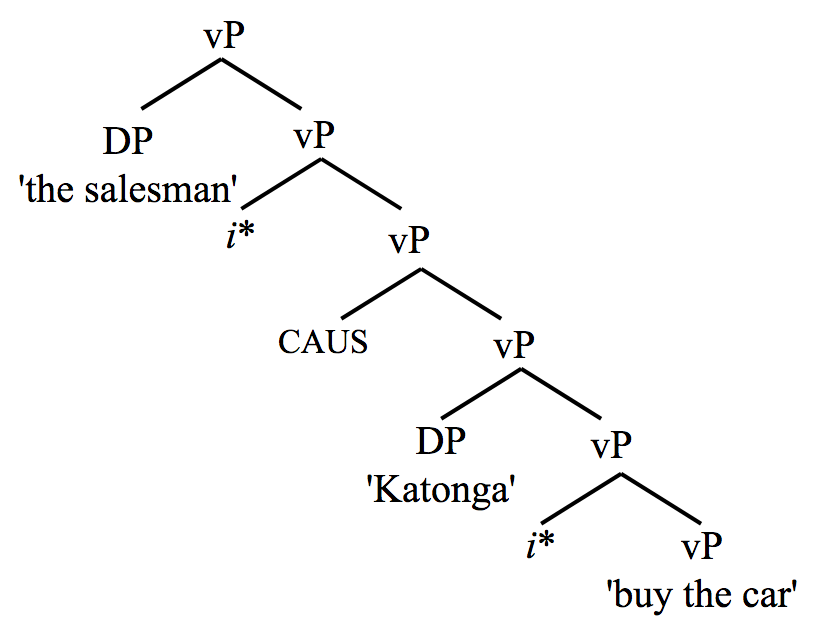
\includegraphics[width=3.2437in,height=2.4484in,width=\textwidth]{wechsler-img003.png}
   [Warning: Image ignored] % Unhandled or unsupported graphics:
%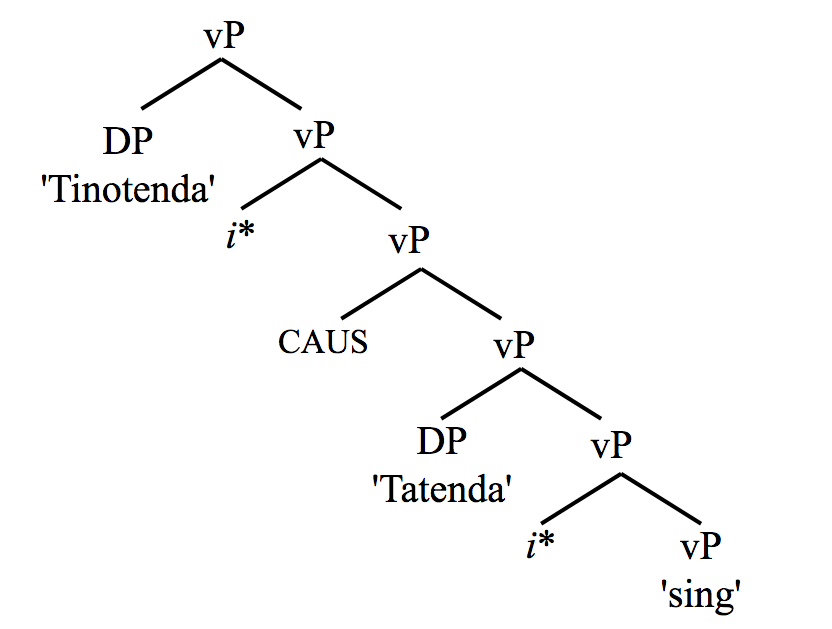
\includegraphics[width=3.2311in,height=2.439in,width=\textwidth]{wechsler-img004.png}
 
\end{styleDefault}

\begin{styleDefault}
\textit{Figure 2: The identical structures of Venda and Shona causatives }
\end{styleDefault}

\begin{styleDefault}
The only difference between the structures in Figure 2 (besides the presence of a DO) is that the lower \textit{i}* in the Venda sentence, which introduces the Agent, \textit{Katonga}, is non-expletive, and the lower \textit{i}* in the Shona sentence, which introduces the non-Agent, \textit{Tatenda}, is expletive. 
\end{styleDefault}


\setcounter{listWWNumxxiileveli}{0}
\begin{listWWNumxxiileveli}
\item 

\setcounter{listWWNumxxiilevelii}{0}
\begin{listWWNumxxiilevelii}
\item 
\begin{stylelsSectionii}
Thematic weight 
\end{stylelsSectionii}
\end{listWWNumxxiilevelii}
\end{listWWNumxxiileveli}
\begin{styleDefault}
In §2.1, I argued that causatives have a maximum “compliment size” restriction, rather than a specific categorial mandate. I propose now that the “size” of a compliment is determined by what I call \textsc{thematic weight. }Thematic weight is the sum of the thematic value of every (non-prepositional) nominal argument in a given constituent. I quantify the thematic value of an argument based on its semantic role, with Agents having the highest value and Themes (or Patients) having the lowest. Thematic hierarchies have been proposed by many authors (Jackendoff 1972, Belletti \& Rizzi 1988, and Grimshaw 1990, to name a few) and while these proposals differ in a number of ways, I follow the general consensus and assume the broad ordering in (\ref{bkm:Ref515944216})\ is sufficient.
\end{styleDefault}


\setcounter{listWWNumiileveli}{0}
\begin{listWWNumiileveli}
\item 
\begin{stylelsLanginfo}
\label{bkm:Ref515944216}\textbf{Agent{\textgreater}Experiencer/Goal{\textgreater}Theme/Patient}
\end{stylelsLanginfo}
\end{listWWNumiileveli}
\begin{styleDefault}
In §2.1 I demonstrated that Causees can occur in any of the three thematic tiers in (\ref{bkm:Ref515944216}). In the Venda sentence in (\ref{bkm:Ref516386347})\ the Causee is an Agent, in the Shona sentence in (\ref{bkm:Ref516385492})\ the Causee is an Experiencer,\footnote{ The traditional definition of “Experiencer” is not a perfect fit for non-agentive Causees of this variety, but because I want to avoid getting bogged down in the profligate lists of thematic relations available in the literature, and also because, for my analysis, the hierarchical tier is more important than the role itself, I consider the imprecision of this and other thematic labels to be acceptable compromises at the present. \par } and in the Bemba sentence in (\ref{bkm:Ref516386265})\ the Causee is a Patient. For the purposes of calculating thematic weight, I assign numerical values to each of the thematic tiers from (\ref{bkm:Ref515944216})\ in Table 1. 
\end{styleDefault}

\begin{flushleft}
\tablefirsthead{}
\tablehead{}
\tabletail{}
\tablelasttail{}
\begin{supertabular}{m{1.1011599in}m{2.08936in}m{1.4476599in}}
\centering Agent &
\centering Experiencer/Goal/Benefactive &
\centering\arraybslash Theme/Patient\\\hline
\centering 3 &
\centering 1 &
\centering\arraybslash 0\\
\end{supertabular}
\end{flushleft}
\begin{styleDefault}
Table 1: Numerical values of thematic roles
\end{styleDefault}

\begin{styleDefault}
Note that these values are stipulative. Multiple authors, Wunderlich (1997) and Mylne (1999), among them, have proposed feature-based decompositions of thematic roles, and more targeted research of this sort could provide a path towards an improved formalization of thematic weight. Furthermore, it is quite possible that the relative weightiness of these roles, as well as which properties and features are grammaticalized as weighty, represents a source of parametric variation. Therefore, the values in Table 1 are merely a starting point.\newline
\newline
I propose that Shona causative heads take compliments with a maximum thematic weight of 2, and that Venda causatives take compliments with a maximum thematic weight of 4 (or potentially more\footnote{ I propose the maximum thematic weight of 3 for compliments of Shona causatives based partially on Wechsler (2014), which explores limitations on the total number of arguments Shona verbs are able to sustain. Without data on the extent to which Venda allows co-occurring causative and applicative heads, I am unable to make an equally precise claim about its causative compliment selection. }). Therefore, any compliment with an Agent is too thematically heavy for a Shona causative to embed. When \textit{i}* introduces non-agentive Causees in unergative and transitive constructions in Shona, it has an expletive interpretation because otherwise it would introduce an Agent, which would render the compliment incompatible with the weight limit of Shona causatives. I also assume that the causative head introduces a Causee and Causer role, and that the Causee role provides the semantic pretense necessary for the expletively-introduced non-Agentive Causee to be integrated into the construction. 
\end{styleDefault}

\begin{styleDefault}
My thematic weight proposal is far more semantically motivated than previous treatments of compliment selection in causative constructions. The Shona sentences in (\ref{bkm:Ref516387012})\ help justify this departure.
\end{styleDefault}

\begin{listWWNumiileveli}
\item 
\begin{stylelsLanginfo}
\label{bkm:Ref516387012}Shona
\end{stylelsLanginfo}
\end{listWWNumiileveli}
\begin{flushleft}
\tablefirsthead{}
\tablehead{}
\tabletail{}
\tablelasttail{}
\begin{supertabular}{m{0.24905986in}m{0.89555985in}m{1.9837599in}m{0.10875984in}m{0.42055985in}m{0.04695984in}m{0.17125985in}m{0.17125985in}m{0.9837598in}}
a. &
{\itshape Tinotenda} &
{\itshape a-ka-donh-es-es-a} &
\multicolumn{3}{m{0.7337598in}}{{\itshape Tatenda}} &
\multicolumn{2}{m{0.42125985in}}{{\itshape poto}} &
{\itshape ye-mvura}\\
 &
1.Tinotenda \  &
\textsc{sm}1-\textsc{pst}{}-fall-\textsc{caus}{}-\textsc{caus}{}-\textsc{fv} &
\multicolumn{3}{m{0.7337598in}}{1.Tatenda} &
\multicolumn{2}{m{0.42125985in}}{9.pot} &
\textsc{poss}{}-9.water\\
 &
\multicolumn{8}{m{5.33306in}}{‘Tinotenda made Tatenda drop the water pot.’

(Litterally: ‘Tinotenda made Tatenda make the water pot fall.’)}\\
b. &
\textit{Tinotenda} &
{\itshape a-ka-dy-is-is-a} &
\multicolumn{2}{m{0.6080598in}}{{\itshape mwana}} &
\multicolumn{4}{m{1.6094599in}}{{\itshape chipunhu}}\\
 &
1.Tinotenda \  &
\textsc{sm}1-\textsc{pst}{}-eat-\textsc{caus}{}-\textsc{caus}{}-\textsc{fv} &
\multicolumn{2}{m{0.6080598in}}{1.child} &
\multicolumn{4}{m{1.6094599in}}{7.spoon}\\
 &
\multicolumn{8}{m{5.33306in}}{‘Tinotends fed the child with a spoon.’

(Literally: ‘Tinotenda made spoon make the child eat.’)}\\
c. &
?\textit{Tinotenda} &
\multicolumn{2}{m{2.1712599in}}{\textit{a-ka-tamba-is-is-a}} &
\multicolumn{3}{m{0.7962598in}}{\textit{Tatenda}} &
\multicolumn{2}{m{1.2337599in}}{\textit{Tendai}}\\
 &
1.Tinotenda \  &
\multicolumn{2}{m{2.1712599in}}{\textsc{sm}1-\textsc{pst}{}-dance-\textsc{caus}{}-\textsc{caus}{}-\textsc{fv}} &
\multicolumn{3}{m{0.7962598in}}{1.Tatenda} &
\multicolumn{2}{m{1.2337599in}}{1.Tendai}\\
 &
\multicolumn{8}{m{5.33306in}}{‘Tinotenda made Tatenda make Tendai dance.’}\\
\end{supertabular}
\end{flushleft}
\begin{stylelsLanginfo}
Each of the sentences in (\ref{bkm:Ref516387012})\ are double-causative constructions. Although \textit{poto yemvura}, ‘water pot’ is the Causee of the first causative in (\ref{bkm:Ref516387012}). It is also the internal argument of the verb and a prototypical Patient so its thematic value is 0. The second Causee \textit{Tatenda} is a non-agentive Experiencer and its thematic value is 1, making the thematic weight of each compliment acceptably light for both causatives to embed. (\ref{bkm:Ref516387012})\ demonstrates that Shona, like Kinyarwanda, exhibits causative-instrumental syncretism (Kimenyi 1980, 1995; Peterson 2007; Jerro 2013). I follow Jerro (2013) and assume that instrumental-causative constructions are not fundamentally different from other causatives. The verb in (\ref{bkm:Ref516387012})\ is transitive, but with its internal argument omitted, rendering the structure essentially identical to the doubly-causativized unegative in (\ref{bkm:Ref516387012}). However, (\ref{bkm:Ref516387012})\ is completely grammatical, whereas (\ref{bkm:Ref516387012})\ is borderline acceptable at best. The problem is thematic weight. In (\ref{bkm:Ref516387012}), the first Causee, \textit{mwana}, ‘the child,’ is non-agentive and has a thematic value of 1, as does the second Causee, \textit{chipunhu}, ‘the spoon.’ The first causative’s compliment has a thematic weight of 1, and the second causative’s compliment has a thematic weight of 2, so neither causative is overburdened and the sentence is grammatical and felicitous. In (\ref{bkm:Ref516387012}), however, it is unintuitive to interpret an animate Causer such as \textit{Tatenda}, as non-agentive, and if \textit{Tatenda} is an Agent, then the thematic weight of the second causative’s compliment is 4, which is far too heavy for a Shona causative head to embed. Although it is unintuitive that \textit{Tatenda} would be non-agentive, it is not impossible. Narrative context that firmly establishes both \textit{Tatenda} and \textit{Tendai} as non-agentive drastically improves the sentences acceptability for my consultant\footnote{ I used a story where Tatenda was under a spell and Tendai was the name of a puppet. }, which further supports my claim that causative selectional restrictions are thematically motivated. While thematic weight may not be the whole story, the sentences in (\ref{bkm:Ref516387012})\ provide strong evidence that some formalized measure of thematic prominence is likely a significant part of the explanation.
\end{stylelsLanginfo}


\setcounter{listWWNumxxiileveli}{0}
\begin{listWWNumxxiileveli}
\item 

\setcounter{listWWNumxxiilevelii}{0}
\begin{listWWNumxxiilevelii}
\item 
\begin{stylelsSectionii}
\textit{i}*-bundling
\end{stylelsSectionii}
\end{listWWNumxxiilevelii}
\end{listWWNumxxiileveli}
\begin{styleDefault}
In addition to compliment selection, Pylkkänen’s causatives are distinguished by a “Voice-bundling” toggle. I assert that this property, which I reconceive as \textit{i}*-bundling, is the product of the causative head merging directly with \textit{i}* before merging into the rest of the structure. The result is that the new compound \textsc{caus}{}-\textit{i}* possesses the selectional requirements of both the causative head and of \textit{i}*. The compound takes an initial compliment according to its inherent thematic weight limit, and because \textit{i}* selects for the category D (Wood \& Marantz 2017: 257) and has not yet had its selectional feature checked, an external argument must be introduced. It is not a property of \textit{i}* that it forces a merge with a nominal argument (Wood \& Marantz 2017: 257), but I argue that when its features bundle with causatives, the resulting structure either mandates the introduction of an agentive external argument or closes off the extended projection of the verbal domain such that no other argument can be merged and semantically integrated. While compliment selection constrains what causatives can embed, \textit{i}*-bundling essentially constrains what can embed causatives. 
\end{styleDefault}

\begin{styleDefault}
Pylkkänen classifies English causatives as “root-selecting” and “Voice-bundling, ” so under this analysis an \textit{i}*-bundling causative that can take compliments with a maximum thematic weight of 0. An English causative cannot embed unergative or transitive roots, because once it has merged, there is no room for anything except the Causer. Because it is non-\textit{i}*-bundling, the Japanese causative can occur with ungergative and transitive roots, despite it also having a maximum compliment weight of 0: 
\end{styleDefault}


\setcounter{listWWNumiileveli}{0}
\begin{listWWNumiileveli}
\item 
\begin{stylelsLanginfo}
\label{bkm:Ref516428768}Japanese (Pylkkänen 2008: 120)
\end{stylelsLanginfo}
\end{listWWNumiileveli}
\begin{flushleft}
\tablefirsthead{}
\tablehead{}
\tabletail{}
\tablelasttail{}
\begin{supertabular}{m{0.76225984in}m{0.76295984in}m{1.0025599in}}
\textit{John-ga} &
\textit{kodomo-o} &
\textit{nak-asi-ta}\\
John-\textsc{nom} &
child-\textsc{acc} &
cry-\textsc{caus-pst}\\
\multicolumn{3}{m{2.6852598in}}{‘John made the child cry.’}\\
\end{supertabular}
\end{flushleft}
\begin{styleDefault}
Figure 3 demonstrates the proposed structure of the sentence in (\ref{bkm:Ref516428768})
\end{styleDefault}

\begin{styleDefault}
\ \   [Warning: Image ignored] % Unhandled or unsupported graphics:
%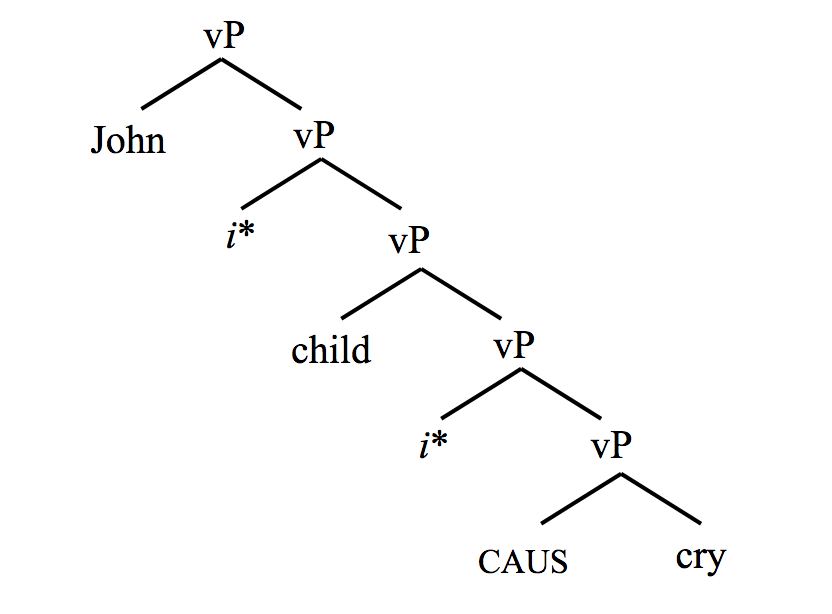
\includegraphics[width=3.0583in,height=2.2575in,width=\textwidth]{wechsler-img005.png}
 
\end{styleDefault}

\begin{styleDefault}
\textit{Figure 3: The structure of a causativized unergative in Japanese}
\end{styleDefault}

\begin{styleDefault}
Figure 3 reveals a problem: the current theory does not prevent the lower \textit{i}* from manifesting non-expletively and introducing an agentive Causee. Like in Shona, Causees in Japanese are non-agentive (Pylkkänen 2008: 107), so in order not to over-generate, this model needs an additional component. I suggest that the first agentive argument to merge above a causative head automatically saturates the Causer role it introduces, closing the structure off to possible Causees. The ‘child’ is therefore non-agentive, because in order to be the Causee and not the Causer, it must be. 
\end{styleDefault}

\begin{styleDefault}
Pylkkänen (2008) asserts that Bemba causatives cannot embed high applicative arguments because they are “verb-selecting” and high applicatives are phase heads, but this conclusion conflicts with the fact that Shona’s “verb-selecting” causatives can embed high applicatives. Pylkkänen cites a Bemba construction where the causative scopes over the applicative and does not address whether or not Bemba also prohibits constructions in which the applicative scopes over the causative. My proposal can account for both of these possibilities, while also accounting for Shona. 
\end{styleDefault}

\begin{styleDefault}
If Bemba allows applicatives to embed causatives, but not vice-versa, its causative selects for compliments with a maximum thematic weight of 1 and does not bundle with \textit{i}*. In this scenario, the causative can embed no more than its non-agentive Causee and a weightless Theme/Patient, which is why complements with Benefactives and co-occurring non-agentive Causees are too heavy. Because the occasion of the causative’s merge does not mandate the immediate introduction of the Causer, however, high applicatives are able to scope over causatives. 
\end{styleDefault}

\begin{styleDefault}
If Bemba completely prohibits causative-applicative co-occurrence, its causative head selects for compliments with a maximum thematic weight of 1 and bundles with \textit{i}*. The causative head is unable to embed applied objects for the same reason as before, but because this causative also necessarily triggers the introduction of an agentive Causer, there is no position for the high applicative to merge and embed it. 
\end{styleDefault}

\begin{styleDefault}
In Hiaki, an Uto-Aztecan language, causatives can embed high applicatives, but high applicatives cannot embed causatives (Jung 2014). An \textit{i}*-bundling causative head that takes compliments with a maximum thematic weight of 2 would be consistent with this causative-applicative co-occurrence pattern. This causative head would be able to embed compliments as large as a non-agentive Causee and an applied object together, but if it were also \textit{i}*-bundling, applicatives would not be able to embed it, because it would be immediately followed by the introduction of an agentive Causer. Since a thorough engagement with Jung (2014) would represent too large a digression, however, all this is merely conjecture, based solely on the scopal possibilities of cooccurring causative-applicative constructions. 
\end{styleDefault}

\begin{styleStandard}
Overall, my proposal, with its three main components, compliment selection based on thematic weight, \textit{i}*-bundling, and the first-Agent-is-the-Causer rule, is both flexible and constrained enough to account for a range of causative variation. 
\end{styleStandard}


\setcounter{listWWNumxxiileveli}{0}
\begin{listWWNumxxiileveli}
\item 
\begin{stylelsSectioni}
Applicatives
\end{stylelsSectioni}


\setcounter{listWWNumxxiilevelii}{0}
\begin{listWWNumxxiilevelii}
\item 
\begin{stylelsSectionii}
Pylkänen’s typology
\end{stylelsSectionii}
\end{listWWNumxxiilevelii}
\end{listWWNumxxiileveli}
\begin{styleStandard}
\newline
Since Pylkkänen first proposed her high-low typology of applicatives (2002) many authors have suggested that this binary is not enough to capture the range of applicative argument introduction in the world’s languages (Jeong 2007; Peterson 2007; Georgala, Paul \& Whitman 2008; Cuervo 2003, 2010, 2012, 2015; Tsai 2009; Kim 2011, 2012; Georgala 2012). In Cuervo’s overview at the beginning of this volume, she presents evidence that far more complexity is necessary to describe the world’s dative and applicative diversity. She proposes a rich typology that takes into account the many kinds of structures that applicatives embed, as well as the many kinds of structures that embed applicatives. It is also my view that Pylkkänen’s model is not fully comprehensive, and in this section, I argue that high and low merge locations are not sufficient to describe the range of applicative constructions in and outside of Bantu. 
\end{styleStandard}

\begin{styleDefault}
Pylkkänen (2008) proposes that there are \textsc{high} and \textsc{low }applicatives. High applicatives are functional heads that introduce and license non-core\textsc{ }arguments merged above the verb and below Voice, relating the applied argument to an event. High applicatives often convey the notion of a favor, where the applied object, prototypically (though not always) a Benefactive, is positively impacted by the entire set of circumstances described by the verb:
\end{styleDefault}


\setcounter{listWWNumiileveli}{0}
\begin{listWWNumiileveli}
\item 
\begin{stylelsLanginfo}
Shona
\end{stylelsLanginfo}
\end{listWWNumiileveli}
\begin{flushleft}
\tablefirsthead{}
\tablehead{}
\tabletail{}
\tablelasttail{}
\begin{supertabular}{m{0.7761598in}m{1.5455599in}m{0.6712598in}m{0.6712598in}}
{\itshape Musikana} &
\textit{a-ka-chek-er-a \ \ \ \ \ \ \ \ \ \ \ \ \ \ \ \ } &
{\itshape baba \ \ \ \ \ \ \ } &
{\itshape uswa}\\
1.girl \ \textsc{\ } &
\textsc{sm1}{}-\textsc{pst}{}-cut-\textsc{appl-fv }\ \  &
1a.father &
14.grass\\
\multicolumn{4}{m{3.9004598in}}{‘The girl cut grass for the father.’}\\
\end{supertabular}
\end{flushleft}
\begin{styleDefault}
Low applicatives introduce and license a non-core argument merged below the verb and relate the applied argument to the verb’s DO. This structure is often interpreted as a transfer of possession: 
\end{styleDefault}

\begin{listWWNumiileveli}
\item 
\begin{stylelsLanginfo}
Shona
\end{stylelsLanginfo}
\end{listWWNumiileveli}
\begin{flushleft}
\tablefirsthead{}
\tablehead{}
\tabletail{}
\tablelasttail{}
\begin{supertabular}{m{0.7754598in}m{1.0462599in}m{0.7969598in}m{0.5455598in}}
{\itshape Mai} &
\textit{va-p-a \ \ \ \ \ \ \ \ \ \ \ \ \ \ \ } &
{\itshape vana \ \ \ \ \ \ \ } &
{\itshape bhuku}\\
2b.mother &
\textsc{sm2}b-give-\textsc{fv} \  &
2.children &
5.book\\
\multicolumn{4}{m{3.4004598in}}{‘The mother gave the children a book.’}\\
\end{supertabular}
\end{flushleft}
\begin{styleDefault}
For Wood \& Marantz, low applicatives are the result of \textit{i}* merging with the internal argument of a verb and introducing another argument interpreted to be the internal argument’s possessor. This merge location is wholly unique to low applicative constructions, so no disambiguating mechanics are necessary; if \textit{i}* merges directly with a nominal argument inside a VP, it always has a low applicative interpretation (see Figure 5). 
\end{styleDefault}

\begin{styleDefault}
  [Warning: Image ignored] % Unhandled or unsupported graphics:
%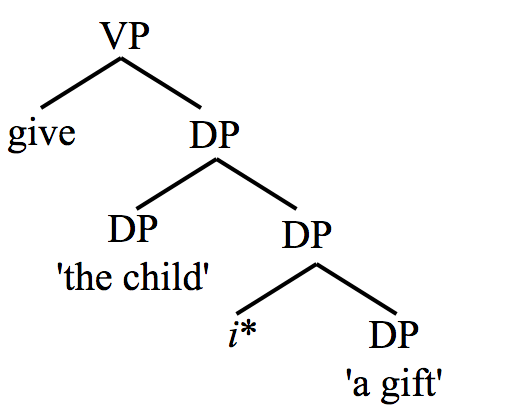
\includegraphics[width=2.0484in,height=1.6339in,width=\textwidth]{wechsler-img006.png}
 
\end{styleDefault}

\begin{styleDefault}
\textit{Figure 5: Partial structure of the low }\textsc{appl}\textit{ construction ‘Miriam gave the children a gift.’}
\end{styleDefault}

\begin{styleDefault}
High applicatives involve the root-adjunction structure I mentioned in my explanation of \textit{i}*-bundling in §2.2. Because the structural position of high applicatives is the same as Voice, Wood \& Marantz distinguish external arguments with high applicative interpretations from external arguments with agentive (or expletive) interpretations, by proposing that before merging with the verb, applicative heads merge with a root that essentially has the meaning of the preposition \textit{for}. In another paper from this collection, Calindro, who also deploys the underspecified \textit{i}* head in her analysis, argues that a curious diachronic shift has occurred in Brazilian Portuguese. The language lacks a lexical root of the kind described by Wood \& Marantz, but Calindro presents evidence that speakers have innovated a construction where \textit{i*} merges with an existing preposition before that combined constituent merges with the verb phrase, a structure nearly identical to the one Wood \& Marantz propose for applicatives (see Figure 6). 
\end{styleDefault}

\begin{styleDefault}
  [Warning: Image ignored] % Unhandled or unsupported graphics:
%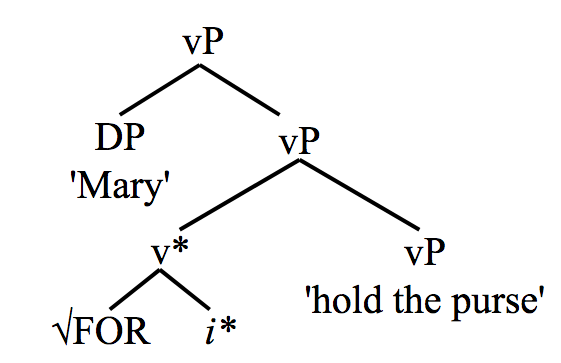
\includegraphics[width=2.1445in,height=1.3862in,width=\textwidth]{wechsler-img007.png}
 
\end{styleDefault}

\begin{styleDefault}
\textit{Figure 6: Partial structure of the high }\textsc{appl}\textit{ construction ‘John held the purse for Mary.’}
\end{styleDefault}

\begin{styleDefault}
In §3.2, I discuss different interpretations of the same applicative surface structure. 
\end{styleDefault}


\setcounter{listWWNumxxiileveli}{0}
\begin{listWWNumxxiileveli}
\item 

\setcounter{listWWNumxxiilevelii}{0}
\begin{listWWNumxxiilevelii}
\item 
\begin{stylelsSectionii}
Applicative Allosemy
\end{stylelsSectionii}
\end{listWWNumxxiilevelii}
\end{listWWNumxxiileveli}
\begin{styleDefault}
The sentence in (\ref{bkm:Ref516387294})\ has three distinct interpretations. 
\end{styleDefault}


\setcounter{listWWNumiileveli}{0}
\begin{listWWNumiileveli}
\item 
\begin{stylelsLanginfo}
\label{bkm:Ref516387294}Shona
\end{stylelsLanginfo}
\end{listWWNumiileveli}
\begin{flushleft}
\tablefirsthead{}
\tablehead{}
\tabletail{}
\tablelasttail{}
\begin{supertabular}{m{0.7768598in}m{1.7323599in}m{0.6087598in}m{0.6087598in}}
\textit{Mai} &
\textit{va-ka-bik-ir-a \ \ \ \ \ \ \ \ \ \ \ \ \ \ \ } &
\textit{mwana} &
\textit{chikafu}\\
2b.mother &
\textsc{sm2}b-\textsc{pst-}cook\textsc{{}-appl}{}-\textsc{fv} \  &
1.child &
7.food\\
\multicolumn{4}{m{3.9629598in}}{i. ‘The mother cooked the child food.’

ii. ‘The mother cooked food for the child.’

iii. ‘The mother cooked the food instead of the child.’}\\
\end{supertabular}
\end{flushleft}
\begin{styleDefault}
Distinguishing between all three meanings is difficult, but narrative context allows for clearer elicitation and explanation of the data. Below are three narratives I used with my consultant to determine that each of these interpretations are valid and possible. 
\end{styleDefault}

\begin{listWWNumiileveli}
\item 
\begin{stylelsLanginfo}
\label{bkm:Ref516387337}\textbf{Recipient}
\end{stylelsLanginfo}
\end{listWWNumiileveli}
\begin{stylelsLanginfo}
The child was hungry and unable to feed herself. Her \textit{mother cooked the child food} and she (the child) ate it. 
\end{stylelsLanginfo}

\begin{styleDefault}
In this interpretation, the applicative defines a relationship between the food the mother cooked and the child. The child receives and then possesses the food. 
\end{styleDefault}

\begin{listWWNumiileveli}
\item 
\begin{stylelsLanginfo}
\label{bkm:Ref516387325}\textbf{Benef}\textbf{active}
\end{stylelsLanginfo}
\end{listWWNumiileveli}
\begin{stylelsLanginfo}
The child was old enough to learn how to cook. She wanted to watch her mother prepare her favorite dish. The mother complied with this wish and \textit{cooked the food for the child} so that she could learn. 
\end{stylelsLanginfo}

\begin{styleDefault}
In this interpretation, the applicative defines a relationship between the child and the event of the food being cooked. The child benefits from the event in a way that does not semantically necessitate the food entering her possession. 
\end{styleDefault}

\begin{listWWNumiileveli}
\item 
\begin{stylelsLanginfo}
\textbf{Substitutive }
\end{stylelsLanginfo}
\end{listWWNumiileveli}
\begin{stylelsLanginfo}
The child was supposed to cook dinner for the family, but she was sick and unable to fulfill her responsibility. The mother helped and \textit{cooked the food instead of the child}, such that she did not have to cook the food. 
\end{stylelsLanginfo}

\begin{styleDefault}
The allosemy in (\ref{bkm:Ref516387337})and (\ref{bkm:Ref516387325})\ is not well accounted for in the literature. Bantu languages have been analyzed as having both (high) applicative derivational morphology and (low) applicative lexical ditransitive constructions (van der Wal 2017). While it is true that all of Bantu’s rare ditransitive roots have low applicative interpretations,\footnote{ Rare because many canonical ditransitives such as ‘show,’ ‘tell,’ or ‘send’ are conveyed using applicative or causative constructions. } it is not true that all applicative morphology corresponds to high applicative semantics. I assume that low meaning coincides with low syntax, and that high meaning coincides with high syntax, regardless of surface level representation. Why some low applicative constructions have applicative morphology and some do not is an important question, one that I am unfortunately unable to answer in this paper. Despite these issues, the syntactic distinction between the Recipient and Benefactive meanings in (\ref{bkm:Ref516387337})\ and (\ref{bkm:Ref516387325})\ is commonly acknowledged. The structure behind the substitutive interpretation, however, is not well established in the literature, so I justify my choice to classify it as semantically and structurally distinct from other high applicatives in §3.3. 
\end{styleDefault}


\setcounter{listWWNumxxiileveli}{0}
\begin{listWWNumxxiileveli}
\item 

\setcounter{listWWNumxxiilevelii}{0}
\begin{listWWNumxxiilevelii}
\item 
\begin{stylelsSectionii}
Super-high applicatives
\end{stylelsSectionii}
\end{listWWNumxxiilevelii}
\end{listWWNumxxiileveli}
\begin{styleDefault}
Marten \& Kula (2014) suggest a \textsc{super-high} applicative in Bemba with substitutive semantics, distinguished morphologically by the locative clitic =kó:
\end{styleDefault}


\setcounter{listWWNumiileveli}{0}
\begin{listWWNumiileveli}
\item 
\begin{stylelsLanginfo}
Bemba (Marten \& Kula 2014: 22)
\end{stylelsLanginfo}
\end{listWWNumiileveli}
\begin{flushleft}
\tablefirsthead{}
\tablehead{}
\tabletail{}
\tablelasttail{}
\begin{supertabular}{m{0.7775598in}m{2.19556in}m{0.70805985in}}
{\itshape Ábá-icé \ \ \ \ \ } &
\textit{bá-lée-tólók-el-a=kó} &
\textit{bá-mayó}\\
2.children &
\textsc{sm2}{}-\textsc{prog-}jump-\textsc{appl-fv=lc17}  &
2.mother\\
\multicolumn{3}{m{3.8386598in}}{‘The children are jumping for/on behalf of the mother.’}\\
\end{supertabular}
\end{flushleft}
\begin{styleDefault}
Shona is like Bemba and has a morphological strategy for indicating substitutive semantics: 
\end{styleDefault}

\begin{listWWNumiileveli}
\item 
\begin{stylelsLanginfo}
\label{bkm:Ref516387395}Shona 
\end{stylelsLanginfo}
\end{listWWNumiileveli}
\begin{flushleft}
\tablefirsthead{}
\tablehead{}
\tabletail{}
\tablelasttail{}
\begin{supertabular}{m{0.9011598in}m{2.0462599in}m{0.7337598in}m{0.6080598in}}
{\itshape Tinotenda \ \ \ } &
\textit{a-ka-bik-ir-ir-a \ \ \ \ \ \ \ \ \ \ \ \ \ \ \ \ \ \ \ \ \ \ \ \ \ \ \ \ \ \ \ \ } &
\textit{Tatenda} &
{\itshape chikafu}\\
1.Tinotenda &
\textsc{sm1-pst}{}-cook-\textsc{appl-appl-fv} \ \  &
1.Tatenda &
7.food\\
\multicolumn{3}{m{3.8386598in}}{‘Tinotenda cooked food instead of Tatenda.’ \ \ } &
\\
\end{supertabular}
\end{flushleft}
\begin{styleDefault}
The doubled applicative affix in (\ref{bkm:Ref516387395})\ is the clearest way to express this interpretation in Shona,\textstyleFootnoteSymbol{ }but the substitutive meaning can be interpreted from a single applicative (demonstrated in (\ref{bkm:Ref516387294})). There are also double applicative structures where each affix indicates a separate instance of applicativization, and two applicative arguments are introduced (see the discussion of (\ref{bkm:Ref516387486})\ later in this section for an example). 
\end{styleDefault}

\begin{styleDefault}
I adopt Marten's (2016) proposal that the substitutive applicative is super-high because it merges above Voice. In Figure 7, I demonstrate this structure using \textit{i}* to introduce all external arguments. \ 
\end{styleDefault}

\begin{styleDefault}
  [Warning: Image ignored] % Unhandled or unsupported graphics:
%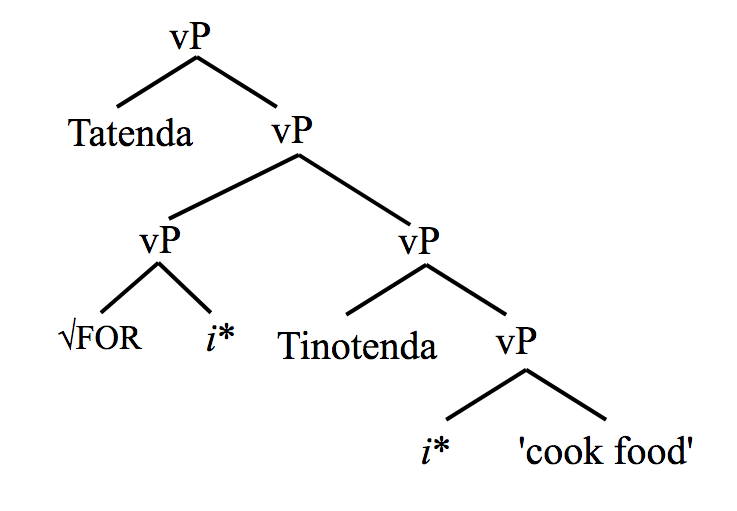
\includegraphics[width=2.8516in,height=1.9756in,width=\textwidth]{wechsler-img008.png}
 
\end{styleDefault}

\begin{styleDefault}
\textit{Figure 7: Structure of the super-high }\textsc{appl }\textit{construction in (\ref{bkm:Ref516387395})}
\end{styleDefault}

\begin{styleDefault}
I assert that super-high applicatives merge first with the same ‘for’ root as high applicatives. The semantic contributions of high and super-high applicatives are similar, in that they both broadly designate the applicative arguments as entities positively impacted by their compliments. Therefore, in combination with the fact that the structural positions of high and super high applicatives are distinct, I argue the same root is sufficient.\newline
\newline
Kim (2011, 2012) also argues for an applicative merge location above Voice (above the external most argument introduced by \textit{i}* in the terms of this analysis). Kim proposes that in Japanese adversity causatives (which I discussed in §2.2) and Korean adversity passives, which are very similar to Japanese adversity causatives an applicative head she calls “peripheral \textsc{appl}” merges very high above all other external arguments and introduces affectee arguments that are the syntactic subjects of their clauses. I assume that, given the similarity between the two structures, Wood \& Marantz’s account of Japanese adversity causatives is a suitable account of Korean adversity passives as well. Kim’s proposed merge location for peripheral \textsc{appl} is motivated primarily by word order: the affectee is the syntactic subject of the construction by virtue of preceding the verb (Korean and Japanese are SOV). In my analysis, the arguments introduced by super-high applicatives are not syntactic subjects and word order is a challenge for the theory, rather than supporting evidence. While I am not able to resolve the issue of word order here,\footnote{ In addition to leaving the derivation of word order to future work, I also beg off the topic of affix ordering. Most Bantu languages have a strict templatic ordering of causative and applicative affixes (Good 2005), and many display causative-applicative co-occurrence with ambiguous scope (Baker 1985; Hyman 2002). It suffices to say, that given variable semantic interpretations and the fact that the causatives and applicatives have to concatenate onto the verb stem apart from the arguments they introduce, movement is necessary to derive these surface structures. Movement is not, however, a part of this analysis. } I do motivate my proposed structural position for super-high applicatives with a variety of evidence. 
\end{styleDefault}

\begin{styleDefault}
Empirical support for the super-high applicative’s super-high merge location in Shona comes from three sources. First, the substitutive semantics relate the applied object, the Substitutee, to the Agent and the entire event in which it participates, indicating that the compliment of the applicative root-adjoined \textit{i}* is large, including the verb phrase and its external argument. \ Second, binding data in double-applicative constructions where there is one substitutive applicative and one high applicative, support the structurally higher placement of the substitutive. 
\end{styleDefault}

\begin{listWWNumiileveli}
\item 
\begin{stylelsLanginfo}
\label{bkm:Ref516387486}Shona
\end{stylelsLanginfo}
\end{listWWNumiileveli}
\begin{flushleft}
\tablefirsthead{}
\tablehead{}
\tabletail{}
\tablelasttail{}
\begin{supertabular}{m{0.21365985in}m{0.42055985in}m{1.6712599in}m{0.6712598in}m{0.42125985in}m{0.26635984in}m{0.20115986in}m{0.39065984in}m{-0.048840158in}m{0.23445985in}m{0.14135984in}m{0.45115986in}}
a. &
\textit{Shiri} &
\textit{\textsubscript{ya-ka-yimb-ir-ir-a }} &
\textit{mai}\textbf{\textit{\textsubscript{i}}} &
\textit{wese} &
\textit{ari} &
\multicolumn{2}{m{0.6705598in}}{\textit{mu-taundi}} &
\multicolumn{3}{m{0.48445985in}}{\textit{mwana}} &
\textit{\textsubscript{w}}\textit{ake}\textbf{\textit{\textsubscript{i}}}\\
 &
9.bird &
\textsc{sm}9-\textsc{pst}{}-sing-\textsc{appl-appl-fv} &
2b.mother\textbf{\textsubscript{i}} &
every &
in &
\multicolumn{2}{m{0.6705598in}}{18-9.town} &
\multicolumn{3}{m{0.48445985in}}{child} &
\textsc{poss}\textbf{\textsubscript{i}}\\
 &
\multicolumn{7}{m{4.51496in}}{‘The bird sang for her\textbf{\textsubscript{i}} child instead of every mother\textbf{\textsubscript{i}} in town.’} &
\multicolumn{3}{m{0.48445985in}}{} &
\\
b. &
{\itshape \textup{*}Shiri} &
{\itshape \ ya-ka-yimb-ir-ir-a} &
{\itshape mai} &
{\itshape wake\textbf{\textsubscript{i}}} &
\multicolumn{2}{m{0.5462598in}}{{\itshape mwana\textbf{\textsubscript{i}}}} &
\multicolumn{2}{m{0.42055985in}}{{\itshape wese}} &
{\itshape ari} &
\multicolumn{2}{m{0.6712598in}}{{\itshape mu-taundi}}\\
 &
9.bird &
\textsc{sm}9-\textsc{pst}{}-sing-\textsc{appl-appl-fv} &
2b.mother &
\textsc{poss}\textbf{\textsubscript{i}} &
\multicolumn{2}{m{0.5462598in}}{child\textbf{\textsubscript{i}}} &
\multicolumn{2}{m{0.42055985in}}{every} &
in &
\multicolumn{2}{m{0.6712598in}}{18-9.town}\\
 &
\multicolumn{11}{m{5.60806in}}{‘The bird sang for every child\textbf{\textsubscript{i}}\textsubscript{~}in town instead of her\textbf{\textsubscript{i}}\textsubscript{ }mother.’}\\
\end{supertabular}
\end{flushleft}
\begin{styleDefault}
In (\ref{bkm:Ref516387486}), the Substitutee (‘the mother’) is able to bind the Benefactive (‘the child’) of the singing event enacted by the Substitute (‘the bird’), but in (\ref{bkm:Ref516387486}), the Benefactive is unable to bind the Substitutee, indicating that the Substitutee is in a higher structural position than the Benefactive. 
\end{styleDefault}

\begin{styleDefault}
I discuss the third source of empirical evidence, which comes from scopal interactions in cooccurring causative-applicative construction, in §3.4.
\end{styleDefault}


\setcounter{listWWNumxxiileveli}{0}
\begin{listWWNumxxiileveli}
\item 

\setcounter{listWWNumxxiilevelii}{0}
\begin{listWWNumxxiilevelii}
\item 
\begin{stylelsSectionii}
Applicative-causative cooccurrence 
\end{stylelsSectionii}
\end{listWWNumxxiilevelii}
\end{listWWNumxxiileveli}
\begin{styleDefault}
Wechsler (2016) concludes that there are four hypothetical scopal interactions in a construction where both an applicative and a causative affix to an unergative stem. They are illustrated with English examples and tree diagrams in Figures 8-12. 
\end{styleDefault}

\begin{styleDefault}
  [Warning: Image ignored] % Unhandled or unsupported graphics:
%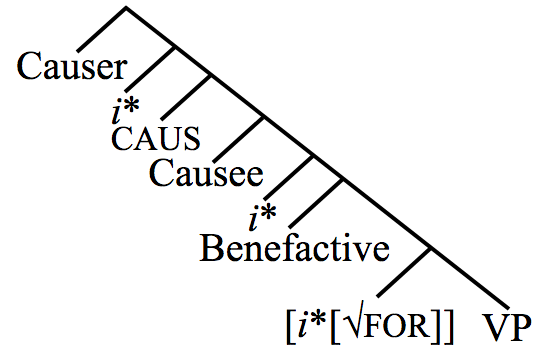
\includegraphics[width=3.0228in,height=1.9744in,width=\textwidth]{wechsler-img009.png}
 
\end{styleDefault}

\begin{styleDefault}
\textit{Figure 8: Causativized high applicative: Tinotenda made Chipo dance for Tatenda (such that Tatenda benefitted from the dancing)}
\end{styleDefault}

\begin{styleDefault}

\end{styleDefault}

\begin{center}
 [Warning: Image ignored] % Unhandled or unsupported graphics:
%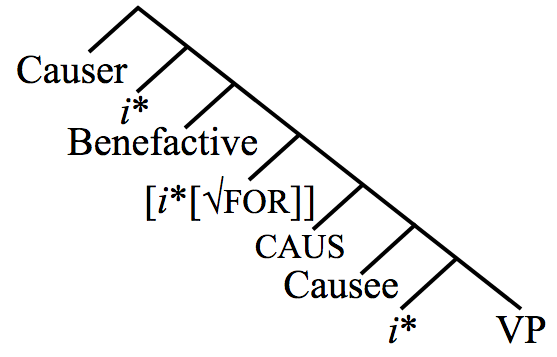
\includegraphics[width=3.0228in,height=1.9354in,width=\textwidth]{wechsler-img010.png}

\end{center}
\begin{styleDefault}
\textit{Figure 9: High applicativized causative: Tinotenda, for Tatenda, made Chipo dance (such that Tatenda benefitted from the coercive action}\footnote{ The interpretive difference between the scopes in Figures 8 and 9 may be difficult to untangle. Imagine, however, a situation where \textit{Tatenda} needs to learn how to make someone dance and so watching \textit{Tinotenda} direct \textit{Chipo} is helpful. }\textit{)}
\end{styleDefault}

\begin{styleDefault}
  [Warning: Image ignored] % Unhandled or unsupported graphics:
%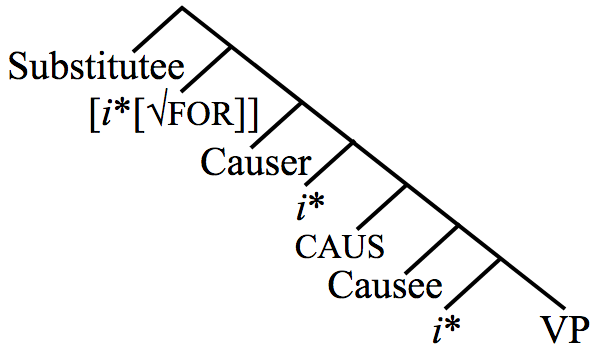
\includegraphics[width=3.0181in,height=1.7902in,width=\textwidth]{wechsler-img011.png}
 
\end{styleDefault}

\begin{styleDefault}
\textit{Figure 10: Super-high applicativized causative: Tinotenda, instead of Tatenda made Chipo dance (such that Tatenda did not have to make Chipo dance)}
\end{styleDefault}

\begin{styleDefault}
  [Warning: Image ignored] % Unhandled or unsupported graphics:
%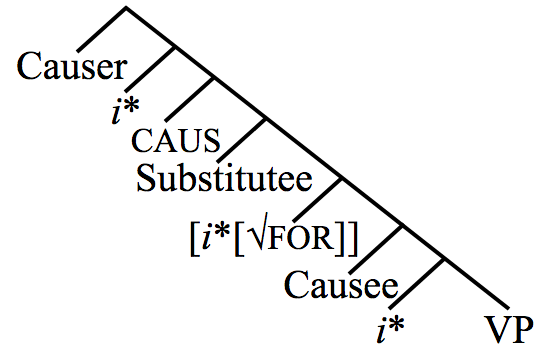
\includegraphics[width=3.0189in,height=1.9752in,width=\textwidth]{wechsler-img012.png}
 
\end{styleDefault}

\begin{styleDefault}
\textit{Figure 11: Causativized Super-high applicative: Tinotenda made Chipo dance instead of Tatenda (such that Tatenda did not have to dance)}
\end{styleDefault}

\begin{styleDefault}
Previously, I stated that the structural positions of high and super-high applicatives were complimentary, but the implementation of \textit{i}* flattens the landscape of structural diversity that anchors the differentiation between the two structures. Super-high applicatives embed external arguments, but Figure 9 demonstrate that high applicatives can embed non-agentive Causees, which are also external arguments, so it is necessary to establish the structural or semantic context that distinguishes super high from high. I assert that when applicative root-adjoined \textit{i}* merges directly above an agentive argument introduced by non-expletive \textit{i}*, it is interpreted as having substitutive semantics. 
\end{styleDefault}

\begin{styleDefault}
Three of the interpretations in Figures 8-11 are possible in Shona. The prohibited interpretation provides the additional evidence I promised in §2.3. Because Shona causatives can embed compliments with a maximum thematic weight of only 2, and because applicative root-adjoined \textit{i}* can only be interpreted as substitutive when it embeds an agentive argument, it follows that Shona causatives would not be able to embed a substitutive applicative. (\ref{bkm:Ref516387563})\ shows that this prediction holds. 
\end{styleDefault}


\setcounter{listWWNumiileveli}{0}
\begin{listWWNumiileveli}
\item 
\begin{stylelsLanginfo}
\label{bkm:Ref516387563}Shona
\end{stylelsLanginfo}
\end{listWWNumiileveli}
\begin{flushleft}
\tablefirsthead{}
\tablehead{}
\tabletail{}
\tablelasttail{}
\begin{supertabular}{m{0.9122598in}m{2.13516in}m{0.8830598in}m{1.5462599in}}
{\itshape Tinotenda \ \ \ } &
\textit{a-tamb-is-ir-a \ \ \ \ \ \ \ \ \ \ \ \ \ \ \ \ \ \ \ \ \ \ \ \ \ \ \ \ \ \ \ \ \ \ \ \ \ \ \ \ \ \ \ \ \ \ \ \ \ \ \ \ \ \ \ \ \ \ \ \ \ \ \ \ \ \ \ \ } &
\textit{Tatenda} &
{\itshape Chipo}\\
1.Tinotenda &
\textsc{sm1-pst}{}-dance-\textsc{caus-appl-fv} \ \  &
1.Tatenda &
1.Chipo\\
\multicolumn{3}{m{4.08796in}}{i. ‘Tinotenda made Chipo, for Tatenda, dance.’ \ \ \ \ \ \ \ \ \ \ \ \ \ \ \ \ \ \ \ \ } &
\textsc{[caus[hi-appl[vP]]]}\\
\multicolumn{3}{m{4.08796in}}{ii. ‘Tinotenda, for Tatenda, made Chipo dance.’} &
\textsc{[hi-appl[caus[vP]]]}\\
\multicolumn{3}{m{4.08796in}}{iii. ‘Tinotenda, instead of Tatenda, made Chipo dance.’} &
\textsc{[sh-appl[caus[vP]]]}\\
\multicolumn{3}{m{4.08796in}}{\textbf{iv. *‘Tinotenda made Chipo, instead of Tatenda, dance.’}} &
\textbf{\textsc{[caus[sh-appl[vP]]]}}\\
\end{supertabular}
\end{flushleft}
\begin{styleDefault}
The Shona causative’s inability to take a substitutive applicative construction as a compliment, demonstrated in (\ref{bkm:Ref516387563})\ by the impossibility of the fourth interpretation, provides robust support for the proposal that substitutive applicatives embed Agents and merge at a higher position than high applicatives. 
\end{styleDefault}

\begin{styleDefault}
Intriguingly, there is a structure in Shona where applicative root-adjoined \textit{i}* heads convey substitutive semantics in a position above a non-agentive argument, and are therefore able to exhibit the generally impossible causativized substitutive interpretation:
\end{styleDefault}

\begin{listWWNumiileveli}
\item 
\begin{stylelsLanginfo}
\label{bkm:Ref516387599}Shona
\end{stylelsLanginfo}
\end{listWWNumiileveli}
\begin{flushleft}
\tablefirsthead{}
\tablehead{}
\tabletail{}
\tablelasttail{}
\begin{supertabular}{m{0.9004598in}m{2.2337599in}m{0.7344598in}}
{\itshape Tinotenda \ \ \ } &
\textit{a-zvi-nyu-dz-ir-a} &
\textit{Tatenda}\\
1.Tinotenda &
\textsc{sm1-refl-}drown\textsc{{}-caus-appl-fv} &
1.Tatenda\\
\multicolumn{3}{m{4.02616in}}{‘Tinotenda made herself drown instead of Tatenda.’\newline
(such that Tatenda did not have to drown) }\\
\end{supertabular}
\end{flushleft}
\begin{styleDefault}
I propose that in (\ref{bkm:Ref516387599}), when the external argument \textit{Tinotenda} is introduced non-expletively as an Agent by \textit{i}*, it saturates three roles in its semantic integration with its compliment. The reflexive morpheme \textit{zvi-} merges in the internal argument position, but only as a place holder that contributes reflexive semantics. When the causative enters the structure, it introduces a Causer and Causee role, and while the internal argument of ‘drown’, would usually saturate the Causee role, the internal argument roles till requires saturation itself. Therefore, when \textit{Tinotenda} merges, it saturates the Causer role, the Causee role, and the Patient role introduced internally by the verb. Because of the unique structure imparted by the reflexive, the applicative root-adjoined \textit{i}* embedded by the causative, though it does not embed an Agent, does embed an argument inextricably related to an Agent, enabling the substitutive interpretation and the usually prohibited scope. This analysis builds on Wood \& Marantz’s (2017) treatment of Icelandic figure reflexives, in which they also propose a structure where an external argument, integrated by non-expletive \textit{i}* as the agentive participant in the event, is identified with a semantic role merged lower in its compliment. 
\end{styleDefault}

\begin{styleStandard}
In this section I have proposed a merge location for applicatives with substitutive semantics, and I have also provided empirical evidence for that structural position. Additionally, I have used the analysis to account for unusual data, showing the theory’s flexibility and strength. §4 concludes. 
\end{styleStandard}


\setcounter{listWWNumxxiileveli}{0}
\begin{listWWNumxxiileveli}
\item 
\begin{stylelsSectioni}
Conclusion
\end{stylelsSectioni}


\setcounter{listWWNumxxiilevelii}{0}
\begin{listWWNumxxiilevelii}
\item 
\begin{stylelsSectionii}
Overgeneration
\end{stylelsSectionii}
\end{listWWNumxxiilevelii}
\end{listWWNumxxiileveli}
\begin{styleStandard}
Overgeneration remains a problem for this analysis. If \textit{i}* is the sole non-core argument introducer in all languages, then why do some languages allow it to merge as a high applicative, and others do not? What about the languages in which \textit{i}* merges even higher with substitutive semantics? Moreover, the disappearance of lexical diversity previously used to formalize argument structure (AS) constraints is globally disruptive to the theory. I am unable to resolve these issues, but my analysis is not alone in retaining this gap.
\end{styleStandard}

\begin{listWWNumxxiileveli}
\item 
\begin{listWWNumxxiilevelii}
\item 
\begin{stylelsSectionii}
Nominal licensing
\end{stylelsSectionii}
\end{listWWNumxxiilevelii}
\end{listWWNumxxiileveli}
\begin{styleDefault}
Kim’s (2011) proposal that unpronounced applicative heads introduce non-agentive Causees is, in some sense, correct, in that both arguments are introduced by \textit{i}* in what could be argued to be its expletive capacity. This begs a question that could provide a very promising seed for further research in the area of dative structures: in what ways are expletive \textit{i}* connected with dative case marking and Case assignment of dative arguments cross-linguistically? 
\end{styleDefault}

\begin{styleDefault}
Many authors build analyses on the assumption that all non-core argument introducers are also sources of abstract Case (Mchombo \& Firmino 1999; Jeong 2007; Cuervo 2003, 2010, 2015; Sheehan 2013; van der Wal 2017) whereas others argue for some degree of decomposition between argument introduction and Case-licensing (Baker \& Collins 2006; Georgala, Paul \& Whitman 2008; Georgala 2012; Haddican \& Holmberg 2012; Halpert 2012; Wechsler 2014, 2016). Additionally, some scholars propose variation in the direction of Case-assignment as another means of accounting for cross-linguistic diversity (Sheehan 2013; van der Wal 2017; Baker 2008). 
\end{styleDefault}

\begin{styleDefault}
Cuervo (2003, 2010) argues that dative subjects of Spanish psychological predicates are licensed by applicative heads, and Royo’s paper in this collection offers a similar account of psych-verbs in Catalan. Kim’s (2011) structurally similar affectee subjects introduced by peripheral \textsc{appl} are nominative, however, with dative marked arguments present elsewhere in the construction. Does expletive \textit{i}* constitute a source of (dative) Case? Perhaps, expletive \textit{i}* introduces affectee subjects in Korean, assigns Case downwards, and licenses an argument it does not introduce, while in Spanish expletive \textit{i}* licenses upwards to reach its introducee. Royo (this volume) argues that Catalan applicative heads can also optionally assign accusative Case (or maybe just license ‘little c’ accusative case), which complicates this hypothesis further. 
\end{styleDefault}

\begin{styleDefault}
If expletive \textit{i}* were\textit{ }a source of dative Case, it would make sense that the various types of dative arguments often bear little semantic resemblance to one another, even intralinguistically. Elsewhere in this volume, Fábregas \& Marín, who argue from a different theoretical perspective, contend that Spanish datives only appear dissimilar and that a single semantic structural property underlies all dative morphology. Were my speculation that dative Case might derive from expletive \textit{i}* true, however, the only semantic property dative-marked arguments would necessarily share is that of being non-agentive (which, it’s worth noting, does not contradict any of the empirical evidence presented by Fábregas \& Marín and especially reflects their data involving the subjects of psychological predicates). 
\end{styleDefault}

\begin{styleDefault}
The literature on applicatives describes a rich AS ecosystem of functional heads that vary with respect to whether they introduce arguments and/or assign Case, as well as whether they assign Case upwards, downwards, or in both directions. How \textit{i}* can be parameterized to capture the breadth of Case-licensing variation is a crucial line of inquiry, with many open questions.
\end{styleDefault}

\begin{listWWNumxxiileveli}
\item 
\begin{listWWNumxxiilevelii}
\item 
\begin{stylelsSectionii}
Parameterization 
\end{stylelsSectionii}
\end{listWWNumxxiilevelii}
\end{listWWNumxxiileveli}
\begin{styleStandard}
One clear advantage that my proposal of causative compliment selection has over prior analyses, is in the arena of parameterization and language acquisition. Rather than individually eliminate every impossible compliment and acquire every possible one, my analysis is such that a child only has to attend to and remember the largest compliment attested in their primary language data, because every smaller (thematically lighter) compliment will be possible. This idea echoes previous work on “implicational hierarchies,” which limit the number of distinct parameters necessary to describe cross-linguistic variation (Holmberg \& Roberts 2009; Biberauer 2011; Biberauer \& Roberts 2012, 2015; Sheehan 2013; Biberauer, Roberts \& Sheehan 2013; van der Wal \& Biberauer 2014; Biberauer et al. 2014; van der Wal 2017).
\end{styleStandard}

\begin{styleStandard}
A potential complication for my proposal, however, is that the choice between expletive and non-expletive interpretation is decided, according to Wood \& Marantz, “in the semantics, after syntactic structure is built and sent to spell-out” (2017: 266). Most of the theoretical stickiness here amounts to an order of operations problem: if the causative head merges before the relevant theta roles in its compliment are assigned, then how can it distinguish based on thematic weight, as I have argued? 
\end{styleStandard}

\begin{styleDefault}
One possibility is that constituent pieces of the structure are sent to spell-out and then semantic interpretation in chunks, a proposal that reflects one of the major concepts of phase theory (Chomsky 1999). This solution represents a compromise between a syntactically-oriented theory of causative compliment selection and a semantically-oriented one, in that the causative head still selects in the syntax, but based on a finalized semantic interpretation that has already been computed at the relevant interface. Another possibility is that what seems like compliment selection is actually an interpretive property that operates after the syntactic derivation. If the latter possibility is correct, where in the grammar is this information stored, and at what point in the derivation does it operate? How is parametric variation in interpretive rules like this captured in the theory? While I do not possess the empirical evidence necessary to settle these issues, my thematic weight proposal ultimately accounts well for the data I have presented, and I leave further theoretical clarification to future work. 
\end{styleDefault}

\begin{listWWNumxxiileveli}
\item 
\begin{listWWNumxxiilevelii}
\item 
\begin{stylelsSectionii}
Summary
\end{stylelsSectionii}
\end{listWWNumxxiilevelii}
\end{listWWNumxxiileveli}
\begin{styleStandard}
In §2, I argued in favor of a single non-core argument introducer, \textit{i}*. I also proposed an original model of compliment selection for causative heads, which accommodates \textit{i}* and reduces the number of individual causative heads necessary to account for intra-linguistic variation. 
\end{styleStandard}

\begin{styleStandard}
In §3, I argued for an additional merge location and associated semantic interpretation for applicative root-adjoined \textit{i}* heads. I also provided empirical evidence for the structural position of super-high applicatives, and offered in depth analysis of causative-applicaitve cooccurrence. 
\end{styleStandard}

\begin{styleStandard}
I have maintained reduction of argument introducers in the lexicon as a priority throughout this analysis. The necessity of more complex compliment selection and a greater number of structural positions for causative and applicative heads does not entail lexical under-specification per se, but it does put into perspective the number of individual functional items that would be required to account for cross-linguistic and intra-linguistic variation in previous analyses. 
\end{styleStandard}

\begin{styleDefault}
I have ultimately provided significant theoretical motivation for a reduced inventory of non-core argument introducers in Bantu, demonstrating that both causative and applicative data can be accommodated by a sparser lexicon. 
\end{styleDefault}

\begin{stylelsSectioni}
Acknowledgments
\end{stylelsSectioni}

\begin{styleStandard}
I want to thank Collence Nyazenga, my dear friend and Shona consultant. I also want to thank Theresa Biberauer for her co-supervision of my master’s thesis (from which much of this analysis developed), and Jenneke van der Wal, who co-supervised my thesis and provided a great deal of feedback on these ideas when they were still in their conference poster infancy. Thank you as well to the editors of this volume for all their hard work, and to my anonymous reviewers for their helpful comments. \ 
\end{styleStandard}

\begin{stylelsSectioni}
Abbreviations
\end{stylelsSectioni}

\begin{styleBody}
\textstyleNone{\textit{In language data from Bantu, numbers and numbers followed by lowercase letters (e.g. 2b) refer to noun classes.}}
\end{styleBody}

\begin{flushleft}
\tablefirsthead{}
\tablehead{}
\tabletail{}
\tablelasttail{}
\begin{supertabular}{m{2.35806in}m{2.35806in}}
\textsc{acc: }accusative &
\textsc{om: }object marker\\
\textsc{appl: }applicative &
\textsc{poss: }possessive\\
\textsc{caus: }causative &
\textsc{prog: }progressive\\
DO\textsc{: }direct object &
\textsc{pst: }past\\
\textsc{dp: }determiner phrase &
\textsc{refl: }reflexive\\
\textsc{fv: }final vowel &
\textsc{sm: }subject marker\\
\textsc{hi-appl: }applicative &
\textsc{sh-appl: }super-high applicative\\
\textsc{inf: }infinitive &
\textsc{vP: }little v phrase\\
\textsc{lc: }locative clitic &
\textsc{VP: }verb phrase\\
\textsc{nom: }nominative &
\\
\end{supertabular}
\end{flushleft}
\begin{stylelsSectioni}
References
\end{stylelsSectioni}

\begin{styleBibliography}
Baker, Mark C. 1985. The Mirror Principle and Morphosyntactic Explanation. \textit{Linguistic Inquiry} 16(3). 373–415.
\end{styleBibliography}

\begin{styleBibliography}
Baker, Mark C. 2008. Parameters of agreement. \textit{The Syntax of Agreement and Concord}, vol. 115, 153–245. (Cambridge Studies in Linguistics). Cambridge, UK: Cambridge University Press.
\end{styleBibliography}

\begin{styleBibliography}
Baker, Mark C. \& Chris Collins. 2006. Linkers and the Internal Structure of vP. \textit{Natural Language \& Linguistic Theory} 24. 307–354.
\end{styleBibliography}

\begin{styleBibliography}
Belletti, Adriana \& Luigi Rizzi. 1988. Psych-Verbs and $\theta $-Theory. \textit{Natural Language \& Linguistic Theory} 6(3). 291–352.
\end{styleBibliography}

\begin{styleBibliography}
Biberauer, Theresa. 2011. In defence of lexico-centric parametric variation: two 3rd factor-constrained case studies. Paper presented at the Workshop on Formal Grammar and Syntactic Variation: Rethinking Parameters, Madrid, ES.
\end{styleBibliography}

\begin{styleBibliography}
Biberauer, Theresa, Anders Holmberg, Ian Roberts \& Michelle Sheehan. 2014. Complexity in comparative syntax: the view from modern parametric theory. In Frederick J. Newmeyer \& Laurel B. Preston (eds.), \textit{Measuring Grammatical Complexity}, 103–127. Oxford, UK: Oxford University Press.
\end{styleBibliography}

\begin{styleBibliography}
Biberauer, Theresa \& Ian Roberts. 2012. On the significance of what hasn’t happened. Conference Presentation. Paper presented at the Diachronic Generative Syntax Conference, Lisbon, PT.
\end{styleBibliography}

\begin{styleBibliography}
Biberauer, Theresa \& Ian Roberts. 2015. Rethinking Formal Hierarchies: A Proposed Unification. \textit{Cambridge Occasional Papers in Linguistics} 7. 1–31.
\end{styleBibliography}

\begin{styleBibliography}
Biberauer, Theresa, Ian Roberts \& Michelle Sheehan. 2013. No-choice Parameters and the Limits of Syntactic Variation. In Robert E. Santana-LaBarge (ed.), \textit{Proceedings of the 31st West Coast Conference on Formal Linguistics}, 46–55. Somerville, MA: Cascadilla Proceedings Project.
\end{styleBibliography}

\begin{styleBibliography}
Chomsky, Noam. 1999. \textit{Derivation by phase}. (MIT Occasional Papers in Linguistics 18). Cambridge, MA: Massachusetts Institute of Technology. 
\end{styleBibliography}

\begin{styleBibliography}
Cuervo, María Cristina. 2003. Datives at Large. Cambridge, MA: Massachusetts Institute of Technology PhD. https://dspace.mit.edu/handle/1721.1/7991.
\end{styleBibliography}

\begin{styleBibliography}
Cuervo, María Cristina. 2010. Some Dative Subjects Are Born, Some Are Made. \textit{Selected Proceedings of the 12th Hispanic Linguistics Symposium}, 13. Somerville, MA: Cascadilla Proceedings Project.
\end{styleBibliography}

\begin{styleBibliography}
Cuervo, María Cristina. 2012. Remarks on Argument Structure. In María Cristina Cuervo \& Yves Roberge (eds.), \textit{The End of Argument Structure?} Bingley, UK: Emerald Group Publishing Limited.
\end{styleBibliography}

\begin{styleBibliography}
Cuervo, María Cristina. 2015. Parameters and Argument Structure II: Causatives and Applicatives. In Antonio Fabregas, Jaume Mateu \& Michael Putnam (eds.), \textit{Contemporary Linguistics Parameters}. Norfolk, UK: Bloomsbury Publishing Plc.
\end{styleBibliography}

\begin{styleBibliography}
Diercks, Michael. 2012. Parameterizing Case: Evidence from Bantu. \textit{Syntax} 15(3). 253–286.
\end{styleBibliography}

\begin{styleBibliography}
Georgala, Efthymia. 2012. Applicatives in their Structural and Thematic Function: A Minimalist Account of Multitransitivity. Cornell University PhD. 
\end{styleBibliography}

\begin{styleBibliography}
Georgala, Efthymia, Waltraud Paul \& John Whitman. 2008. Expletive and Thematic Applicatives. In Charles B. Chang \& Hannah J. Haynie (eds.), \textit{Proceedings of the 26th West Coast Conference on Formal Linguistics}. Somerville, MA: Cascadilla Proceedings Project.
\end{styleBibliography}

\begin{styleBibliography}
Givón, Talmy. 1969. Studies in Chibemba and Bantu Grammar. Los Angeles, CA: University of California, Los Angeles PhD.
\end{styleBibliography}

\begin{styleBibliography}
Good, Jeff. 2005. Reconstructing morpheme order in Bantu: The case of causativization and applicativization. \textit{Diachronica} 22(1). 3–57. 
\end{styleBibliography}

\begin{styleBibliography}
Grimshaw, Jane B. 1990. \textit{Argument structure.} (Linguistic Inquiry Monographs: 18). Cambridge, Mass.[202F?]: MIT Press, c1990. 
\end{styleBibliography}

\begin{styleBibliography}
Haddican, William \& Anders Holmberg. 2012. Object Movement (A)symmetries in British English Dialects. In Jaehoon Choi, E. Alan Hogue, Jeffrey Punske, Deniz Tat, Jessamyn Schertz \& Alex Trueman (eds.), \textit{Proceedings of the 29th West Coast Conference on Formal Linguistics}, 72–80. Somerville, MA: Cascadilla Proceedings Project.
\end{styleBibliography}

\begin{styleBibliography}
Halpert, Claire. 2012. Argument licensing and agreement in Zulu. Cambridge, MA: Massachusetts Institute of Technology.
\end{styleBibliography}

\begin{styleBibliography}
Haspelmath, Martin. 2016. Universals of causative and anticausative verb formation and the spontaneity scale. \textit{Lingua Posnaniensis} 
\end{styleBibliography}

\begin{styleBibliography}
Holmberg, Anders \& Ian Roberts. 2009. Introduction: Parameters in Minimalist Theory. In Theresa Biberauer, Anders Holmberg, Ian Roberts \& Michelle Sheehan (eds.), \textit{Parametric Variation: Null Subjects in Minimalist Theory}, 1–57. Cambridge, UK: Cambridge University Press..
\end{styleBibliography}

\begin{styleBibliography}
Hyman, Larry M. 2002. Suffix ordering in Bantu: a morphocentric approach. In Geert Booij \& Jaap van Marle (eds.), \textit{Yearbook of Morphology 2002}, 245–281. Dordrecht, NL: Kluwer Academic Publishers. 
\end{styleBibliography}

\begin{styleBibliography}
Jackendoff, Ray. 1972. \textit{Semantic interpretation in generative grammar.} (Studies in Linguistics 2). Cambridge, MA: MIT Press. 
\end{styleBibliography}

\begin{styleBibliography}
Jeong, Youngmi. 2007. \textit{Applicatives[202F?]: structure and interpretation from a minimalist perspective.} (Linguistik Aktuel = Linguistics Today: V. 104). Amsterdam[202F?]; Philadelphia[202F?]: John Benjamins Pub. Co., c2007..
\end{styleBibliography}

\begin{styleBibliography}
Jerro, Kyle Joseph. 2013. Argument Structure and the Typology of Causatives in Kinyarwanda: Explaining the Causative-Instrumental Syncretism. Austin, TX: University of Texas at Austin MA.
\end{styleBibliography}

\begin{styleBibliography}
Jung, Hyun Kyoung. 2014. On the Syntax of Applicative and Causative Construction. Tucson, AZ: University of Arizona PhD.
\end{styleBibliography}

\begin{styleBibliography}
Kim, Kyumin. 2011. External Argument Introducers. Toroto, ON: University of Toronto PhD. https://tspace.library.utoronto.ca/handle/1807/31805.
\end{styleBibliography}

\begin{styleBibliography}
Kim, Kyumin. 2012. External Argument-Introducing Heads: Voice and Appl. In María Cristina Cuervo \& Yves Roberge (eds.), \textit{The End of Argument Structure?}, 131–154. Bingley, UK: Emerald Group Publishing Limited. 
\end{styleBibliography}

\begin{styleBibliography}
Kimenyi, Alexandre. 1980. \textit{A Relational Grammar of Kinyarwanda.} Berkeley \& Los Angeles, CA: University of California Press.
\end{styleBibliography}

\begin{styleBibliography}
Kimenyi, Alexandre. 1995. Kinyarwanda applicatives revisited. Conference Presentation. Paper presented at the Niger-Congo syntax and semantics workshop on the applicative architectures, Boston, MA. 
\end{styleBibliography}

\begin{styleBibliography}
Kittilä, Seppo. 2013. Causative morphemes as a de-transitivizing device: what do non-canonical instances reveal about causation and causativization? \textit{Folia Linguistica} 47(1). 113–137. 
\end{styleBibliography}

\begin{styleBibliography}
Marten, Lutz. 2016. Benefactive and substitutive applicatives in Bemba. Paper presented at the Syntax Research Cluster Event, Cambridge, UK.
\end{styleBibliography}

\begin{styleBibliography}
Marten, Lutz \& Nancy C. Kula. 2014. Benefactive and substitutive applicatives in Bemba. \textit{Journal of African Languages and Linguistics} 35(1). 1–44. doi:10.1515/jall-2014-0001.
\end{styleBibliography}

\begin{styleBibliography}
Kulikov, Leonid. 2001. Causatives. In Haspelmath Martin (ed.), \textit{Language Typology and Language Universals: An International Handbook}, vol. 2, 886–898. Berlin, Germany; New York, NY: Walter De Gruyter. 
\end{styleBibliography}

\begin{styleBibliography}
Mchombo, Sam A. \& Gregório Firmino. 1999. Double Object Constructions in Chichewa and Gitonga: A Comparative Analysis. \textit{Linguistic Analysis} 29(1). 214–233.
\end{styleBibliography}

\begin{styleBibliography}
Mylne, Tom. 1999. A Feature-based System for Classifying Semantic Roles. \textit{Proceedings of the 1999 Conference of the Australian Linguistic Society}, 10.
\end{styleBibliography}

\begin{styleBibliography}
Peterson, David A. 2007. \textit{Applicative constructions.} (Oxford Studies in Typology and Linguistic Theory). Oxford, UK; New York, NY: Oxford University Press. 
\end{styleBibliography}

\begin{styleBibliography}
Pylkkänen, Liina. 2002. Introducing Arguments. Cambridge, MA: Massachusetts Institute of Technology PhD.
\end{styleBibliography}

\begin{styleBibliography}
Pylkkänen, Liina. 2008. \textit{Introducing arguments.} (Linguistic Inquiry Monographs 49). Cambridge, MA: MIT Press. 
\end{styleBibliography}

\begin{styleBibliography}
Sheehan, Michelle. 2013.Towards a Parameter Hierarchy for Alignment. Paper presented at the West Coast Conference on Formal Linguistics, Tempe, AZ.
\end{styleBibliography}

\begin{styleBibliography}
Sheehan, Michelle \& Jenneke van der Wal. 2016. Do we need abstract Case? In Kyeong-min Kim, Pocholo Umbal, Trevor Block, Queenie Chan, Tanie Cheng, Kelli Finney, Mara Katz, Sophie Nickel-Thompson \& Lisa Shorten (eds.), \textit{Proceedings of the 33rd West Coast Conference on Formal Linguistics}, 351–360. Somerville, MA: Cascadilla Proceedings Project.
\end{styleBibliography}

\begin{styleBibliography}
Tsai, Wei-Tien Dylan. 2009. High Applicatives are not High Enough: A Cartographic Solution. \textit{6th Workshop on Formal Syntax and Semantics (FOSS-6)}. Taipei, Taiwan: National Taiwan Normal University. 
\end{styleBibliography}

\begin{styleBibliography}
Wal, Jenneke van der. 2015. Evidence for abstract Case in Bantu. \textit{Lingua} 165. 109–132. 
\end{styleBibliography}

\begin{styleBibliography}
Wal, Jenneke van der. 2017. Flexibility in symmetry: An implicational relation in Bantu double object constructions. In Laura R Bailey \& Michelle Sheehan (eds.), \textit{Order and structure in syntax II: Subjecthood and argument structure}, 48. (Order and Structure in Syntax 2). Berlin, Germany: language science press.
\end{styleBibliography}

\begin{styleBibliography}
Wal, Jenneke van der \& Theresa Biberauer. 2014. From Macroparameters to Nanoparamters-A comparative Bantu case study. Conference Presentation. Paper presented at the International Workshop on Bantu Languages: Studies in East African Bantu and Microvariation, London, UK.
\end{styleBibliography}

\begin{styleBibliography}
Wechsler, Mattie. 2014. The Stacking Behavior of Valence-Increasing Verbal Extensions and Their Arguments in Shona. Bryn Mawr College 
\end{styleBibliography}

\begin{styleBibliography}
Wechsler, Mattie. 2016. Case-Assignment in Causative, Applicative, Double Object Constructions: A Comparative Analysis with Emphasis on Micovariation in Bantu. University of Cambridge MPhil.
\end{styleBibliography}

\begin{styleBibliography}
Wood, Jim \& Alec Marantz. 2017. The interpretation of external arguments. In Roberta D’Alessandro, Irene Franco \& Angel J. Gallego (eds.), \textit{The verbal domain}, 255–278. Oxford, UK: Oxford University Press. 
\end{styleBibliography}

\begin{styleBibliography}
Wunderlich, Dieter. 1997. Cause and the Structure of Verbs. \textit{Linguistic Inquiry} 28(1). 27–68.
\end{styleBibliography}

\end{document}
